\documentclass[11pt]{article}
\usepackage[a4paper,margin=25mm]{geometry}
\usepackage{amsmath,amssymb,booktabs,longtable,siunitx,graphicx,xcolor,xurl,hyperref}
\usepackage[numbers,sort&compress]{natbib}
\usepackage[expansion=false]{microtype}
\usepackage{pgfplots,pgfplotstable,tikz}
\usetikzlibrary{arrows.meta,positioning,fit}
\pgfplotsset{compat=1.18}
\sisetup{detect-all}
\title{Nuclear-Assisted Steam Methane Reforming with Carbon Capture in Singapore:\\
A Literature-Anchored Assessment of Process Integration, Emissions and Feasibility}
\author{Nuclear-Assisted Hydrogen Research Project}
\date{}
\begin{document}
\maketitle
\begin{abstract}
Singapore requires low-carbon technologies that can deliver more than 0.25 MtCO$_2$e/y of abatement at less than S\$100/tCO$_2$e. This study evaluates a literature-anchored nuclear-assisted steam-methane-reforming (SMR) plant with carbon capture and storage (CCS). The final process basis is INL's NGNP high-temperature case: an 871$^\circ$C reformer at steam/carbon 3.0, supplied with 900$^\circ$C nuclear process heat from a 925$^\circ$C HTGR outlet, with 78.1\% methane conversion, 88\% PSA recovery and carbon capture~\cite{inltev953,inltev961}. JAEA GTHTR300C evidence supplies the 600 MWth module, helium/IHX architecture and one-module cogeneration economics~\cite{jaeri2004gthtr300c,nishihara2007potential}. At 85\% availability the 130 MMSCFD source service corresponds to approximately 97,946 tH$_2$/y. Extending the source balance with upstream-gas, nuclear-lifecycle, CCS-transport and Singapore economic accounting gives approximately 0.917 MtCO$_2$e/y lifecycle abatement. The conservative zero-value-cogeneration case gives approximately S\$30.2/tCO$_2$e, satisfying the CN4252 cost threshold without electricity revenue; the mature S\$150/MWh screening case gives approximately $-$S\$194.7/tCO$_2$e because modelled annual candidate cost falls below the baseline under that electricity-value assumption. The result is a \textbf{conditional model result}, not observed Singapore commercial feasibility: it depends on mature HTGR design-study economics, an enlarged high-temperature IHX/secondary-loop treatment, cross-border CO$_2$ storage and lifecycle screening proxies.
\end{abstract}

\section*{How to read this paper}
Start with one question: \emph{Can nuclear heat replace the gas-fired heat used to make hydrogen, while carbon capture reduces the remaining emissions, at an acceptable cost?} Sections 1--3 explain the plant and its evidence boundary. Sections 4--8 follow energy, hydrogen and carbon through the process. Sections 9--10 turn the physical results into annual cost and uncertainty. Sections 11--13 answer the Singapore feasibility question and identify what must be proven before deployment.

Each numerical claim has a maturity level: \textbf{source observation} (reported in literature), \textbf{project calculation} (derived from stated inputs), \textbf{scenario} (dependent on assumptions) or \textbf{not demonstrated} (still needs data). In particular, the mature cost is a projected scenario, not today's price. Read the units: MWth is a rate of heat delivery, MWe is electrical power, tCO$_2$/y is a physical carbon-dioxide stream, and tCO$_2$e/y measures greenhouse-gas impact on a lifecycle basis. They are not interchangeable.

\section*{Nomenclature}
\begin{longtable}{p{0.18\linewidth}p{0.72\linewidth}}
\toprule
Symbol / acronym & Definition and units where applicable \\
\midrule
\endfirsthead
\toprule
Symbol / acronym & Definition and units where applicable \\
\midrule
\endhead
SMR & Steam methane reforming; nuclear SMR is written explicitly when referring to a small modular reactor. \\
CCS & Carbon capture and storage. \\
CCUS & Carbon capture, utilisation and storage. \\
WGS & Water--gas shift reaction. \\
PSA & Pressure swing adsorption for hydrogen purification. \\
HTGR & High-Temperature Gas-Cooled Reactor. \\
HTR & High-Temperature Reactor. \\
GTHTR300C & Gas Turbine High-Temperature Reactor 300 for Cogeneration. \\
HTTR & High Temperature Engineering Test Reactor. \\
HTR-PM & High-Temperature Reactor Pebble-bed Module. \\
IHX & Intermediate Heat Exchanger between the reactor primary circuit and secondary heat-transfer loop. \\
TRISO & Tri-structural Isotropic coated fuel particle used in HTGR fuel. \\
EPZ & Emergency Planning Zone. \\
PRA & Probabilistic Risk Assessment. \\
QRA & Quantitative Risk Assessment. \\
LCA & Life-Cycle Assessment. \\
TEA & Techno-Economic Analysis. \\
FOAK & First-of-a-Kind. \\
I\&C & Instrumentation and Control. \\
V\&V & Verification and Validation. \\
LOFC & Loss of Forced Cooling. \\
LOCA & Loss of Coolant Accident. \\
INL & Idaho National Laboratory. \\
JAEA & Japan Atomic Energy Agency. \\
JAERI & Japan Atomic Energy Research Institute. \\
IAEA & International Atomic Energy Agency. \\
IEA & International Energy Agency. \\
UNECE & United Nations Economic Commission for Europe. \\
EMA & Energy Market Authority (Singapore). \\
MTI & Ministry of Trade and Industry (Singapore). \\
NRC & United States Nuclear Regulatory Commission when used in this report. \\
NGNP & Next Generation Nuclear Plant. \\
IEAGHG & IEA Greenhouse Gas R\&D Programme. \\
S/C & Steam-to-carbon molar ratio at the reformer feed. \\
ROT & Reactor outlet temperature. \\
MWth & Megawatt of thermal power (heat rate). \\
MWe & Megawatt of electrical power. \\
T\&S & CO$_2$ transport and geological storage. \\
MDEA & Methyldiethanolamine-based CO$_2$ capture system represented by the source-anchored screening duty. \\
$Q_r$ & Reaction quotient for reaction $r$, dimensionless under the adopted standard-state convention. \\
$K_r(T)$ & Equilibrium constant for reaction $r$ at temperature $T$, dimensionless under the same convention. \\
$\dot n_i$ & Molar flow of species $i$, kmol/h unless otherwise stated. \\
$\dot H$ & Stream enthalpy rate, MW on the model basis. \\
$Q_{\mathrm{ref}}$ & External reformer heat duty, MW. \\
$I_{\mathrm{base}}$ & Baseline lifecycle emissions intensity, kgCO$_2$e/kgH$_2$. \\
$I_{\mathrm{cand}}$ & Candidate lifecycle emissions intensity, kgCO$_2$e/kgH$_2$. \\
$\dot m_{H_2}$ & Hydrogen mass-production rate, kg/h. \\
$t_{\mathrm{op}}$ & Annual operating time, h/y; common IEAGHG basis is 8322 h/y. \\
$E_{\mathrm{avoided}}$ & Annual avoided lifecycle emissions, tCO$_2$e/y after unit conversion. \\
$C_{\mathrm{base}}$ & Annual baseline cost, S\$/y for forward Singapore screening comparisons. \\
$C_{\mathrm{cand}}$ & Annual candidate cost, S\$/y on the same basis. \\
$C_{\mathrm{abatement}}$ & Forward abatement cost, S\$/tCO$_2$e when numerator and denominator share a consistent basis. \\
\bottomrule
\end{longtable}

\section{Introduction and research question}
Hydrogen is an industrial feedstock used in applications such as refining and chemical manufacture. A common production route is steam methane reforming (SMR): natural gas reacts with steam to form a hydrogen-rich synthesis gas. The chemistry and the high-temperature reformer both create a carbon challenge. Carbon entering with methane ultimately appears largely as CO$_2$, while conventional reformers also burn fuel to supply reaction heat.

Carbon capture and storage (CCS) can separate and store much of the concentrated process CO$_2$, but it does not by itself eliminate fired reformer heat or upstream natural-gas emissions. This motivates the question tested here: can high-temperature nuclear heat replace the fired heat service while CCS manages process carbon?

A high-temperature gas-cooled reactor (HTGR) is relevant because helium coolant can deliver temperatures suitable for industrial process heat. An intermediate heat exchanger (IHX) isolates the nuclear primary-helium circuit from a separate secondary-helium circuit feeding the reformer. The proposal therefore transfers heat across an engineered boundary rather than sending reactor primary coolant into the chemical process.

For Singapore, this remains a future-oriented screening question rather than an existing deployment option. Nuclear licensing/siting and cross-border CO$_2$ storage are not established project infrastructure. CN4252 nevertheless supplies a quantitative test: the proposed solution must avoid more than 0.25 MtCO$_2$e/y at an abatement cost below S\$100/tCO$_2$e.

The research question is therefore: \emph{does the strongest directly supported HTGR-assisted SMR+CCS design found in the primary literature satisfy both CN4252 thresholds when its process balance is extended to a transparent Singapore lifecycle and forward-economic boundary?}

The final process basis is INL's NGNP HTGR-integrated SMR analysis~\cite{inltev953,inltev961}; Nishihara/JAEA evidence supplies the selected HTGR/IHX hardware and mature design-study economic architecture~\cite{nishihara2007potential}. Historical project configurations remain in the repository for audit but are not the submission-facing design.

\section{Literature and technical background}
Natural-gas SMR combines high-temperature reforming with water--gas shift (WGS), hydrogen purification and substantial process heat. Literature and authoritative sources establish three facts central to this study: lifecycle emissions cannot be inferred from stack capture alone because upstream natural-gas emissions remain material; high-temperature gas-cooled reactors can provide high-grade helium heat in principle, but reactor-to-chemical-plant coupling remains an integration problem rather than a demonstrated Singapore deployment; and CCS energy and cost depend strongly on the pressure and composition of the captured stream.

The structured literature matrix in \texttt{literature/RESEARCH\_MATRIX.md} records the evidence basis and contradictions used in model construction. International Energy Agency Greenhouse Gas R\&D Programme (IEAGHG) SMR+CCS cases~\cite{ieaghg2017smr} provide the principal process benchmark; National Institute of Standards and Technology (NIST)/JANAF thermochemistry~\cite{nistwebbook} underpins equilibrium and enthalpy calculations; JAEA / Japan Atomic Energy Research Institute (JAERI) HTTR and GTHTR300C work~\cite{jaeahttr,jaeri2004gthtr300c} provides temperature, IHX and helium-loop precedent; Singapore Government sources~\cite{mti2025nuclear,mti2026inir,mti2025carbon,mti2025indonesiaccs} define nuclear and cross-border CCS as future or conditional infrastructure rather than existing assets.



\subsection{Three-figure orientation: baseline, nuclear power, proposed integration}
Before the detailed derivations, Figures~\ref{fig:smr-explainer}--\ref{fig:proposed-orientation} answer three different questions: how conventional hydrogen production obtains reformer heat; what an HTGR normally does with reactor heat in a power-production pathway; and what this project changes by diverting high-temperature heat to the hydrogen process.

\begin{figure}[htbp]\centering
\resizebox{\textwidth}{!}{\input{../results/final_design/generated/figure1_conventional_smr_ccs.tex}}
\caption{Figure 1---conventional hydrogen-production orientation. SMR = Steam Methane Reformer/Reforming; WGS = Water-Gas Shift; CCS = Carbon Capture and Storage; PSA = Pressure Swing Adsorption; T\&S = carbon-dioxide Transport and Storage. The fired furnace supplies the high-temperature reformer heat service; process gas then passes through WGS, CO$_2$ capture and PSA to hydrogen product, while captured CO$_2$ proceeds to conditioning and T\&S. This is an original static engineering schematic reconstructed from the source process; equipment silhouettes are schematic art rather than design drawings~\cite{ieaghg2017smr,inltev953}.}
\label{fig:smr-explainer}
\end{figure}

\begin{figure}[htbp]\centering
\resizebox{0.94\textwidth}{!}{\input{../results/final_design/generated/figure2_htgr_power.tex}}
\caption{Figure 2---conceptual conventional HTGR electricity-generation pathway. HTGR = High-Temperature Gas-Cooled Reactor; He = helium. Primary helium forms a closed reactor-to-steam-generator loop; the separate steam/water cycle drives a turbine and generator and returns condensate through a pump. This is a reference architecture only and does \textbf{not} assign or imply a numerical electricity output for the proposed CN4252 system. Equipment silhouettes are schematic art, not mechanical design drawings.}
\label{fig:htgr-power-orientation}
\end{figure}

\begin{figure}[p]\centering
\resizebox{\textwidth}{!}{\input{../results/final_design/generated/figure3_proposed_htgr_smr_ccs.tex}}
\caption{Figure 3---proposed HTGR-assisted SMR+CCS system. HTGR = High-Temperature Gas-Cooled Reactor; IHX = Intermediate Heat Exchanger; He = helium; SMR = Steam Methane Reformer; WGS = Water-Gas Shift; PSA = Pressure Swing Adsorption; CCS = Carbon Capture and Storage; T\&S = Transport and Storage. Idaho National Laboratory process evidence anchors the 925$^\circ$C reactor-outlet case, 900$^\circ$C secondary-He supply, approximately 466$^\circ$C return, 78.49 kg/s source flow, 871$^\circ$C reformer outlet, 176.8 MWth duty, S/C=3.0 and 88\% PSA hydrogen recovery~\cite{inltev953,inltev961}. The 600 MWth GTHTR300C-class reactor basis is a literature design basis~\cite{jaeri2004gthtr300c,nishihara2007potential}. Primary and secondary helium are physically separated by the IHX and neither mixes with the SMR process gas. The approximately 170 MWth value is a physical-IHX reference/qualification caveat and does not establish a qualified 176.8 MWth project IHX. The approximately 370/371 MWth value is the source architecture/economic process-heat branch, \textbf{not} one physical IHX~\cite{nishihara2007potential}. The 423.2 MWth value is remaining reactor thermal capacity, \textbf{not} electricity output. The 88\% value is PSA hydrogen recovery, \textbf{not} hydrogen purity. H$_2$ product is 130 MMSCFD; annualised output is approximately 97,946 t/y. The CO$_2$ endpoint is a conditional transport/storage screening boundary rather than guaranteed infrastructure.}
\label{fig:proposed-orientation}
\end{figure}

\subsection{How the proposed system works, step by step}
\begin{enumerate}
\item \textbf{Fission produces heat.} Nuclear fission releases energy primarily as fission-fragment kinetic energy and associated energy deposition, heating the reactor fuel and core; subsequent radioactive decay contributes decay heat.
\item \textbf{Primary helium removes core heat.} At the selected process operating point, the source reactor-outlet case is 925$^\circ$C~\cite{inltev961}.
\item \textbf{Primary helium reaches the IHX.} The hot primary coolant carries reactor heat to the Intermediate Heat Exchanger.
\item \textbf{The IHX provides physical separation.} Heat crosses exchanger walls; primary reactor helium does not enter the chemical plant.
\item \textbf{Secondary helium receives the heat.} INL Case 6 supplies secondary helium at 900$^\circ$C with a reported process-side flow of 78.49 kg/s~\cite{inltev961}.
\item \textbf{Secondary helium heats the reformer.} The source process requires 176.8 MWth and reports an 871$^\circ$C reformer outlet~\cite{inltev953,inltev961}.
\item \textbf{Secondary helium returns.} After heat transfer, the source return state is approximately 466$^\circ$C before reheating at the IHX~\cite{inltev961}.
\item \textbf{Natural gas and steam enter the reformer.} The selected steam-to-carbon molar ratio is 3.0~\cite{inltev953}. Nuclear heat replaces fossil \emph{process heat}; natural gas remains the chemical hydrogen feedstock.
\item \textbf{Steam methane reforming produces synthesis gas.} Methane reacts with steam to form a hydrogen-rich mixture containing carbon monoxide.
\item \textbf{Water-gas shift increases hydrogen.} Carbon monoxide reacts with steam toward CO$_2$ and additional H$_2$.
\item \textbf{CO$_2$ is separated.} The source process represents amine-based capture of the concentrated carbon stream.
\item \textbf{PSA recovers hydrogen.} The selected Pressure Swing Adsorption recovery is 88\%~\cite{inltev953}.
\item \textbf{Hydrogen leaves as product.} The source service is 130 million standard cubic feet per day (MMSCFD) H$_2$~\cite{inltev953,inltev961}; annualised at 85\% availability, the project calculation gives approximately 97,946 t H$_2$/y.
\item \textbf{Captured CO$_2$ is conditioned.} The source captured stream is 1,927 short ton/day~\cite{inltev961}, annualised to approximately 542,362 t/y at the declared availability.
\item \textbf{CO$_2$ leaves the project boundary.} Compression/conditioning leads to transport and geological storage; the cross-border route and storage site remain conditional rather than demonstrated.
\end{enumerate}

\subsection{Visual orientation: from Singapore context to the process}
Figure~\ref{fig:singapore-context} gives the external-data context before introducing the process model. Singapore's 2024 electricity system remained strongly gas-dependent: natural gas supplied 94.0\% of the generation fuel mix and the average grid emission factor was 0.402 kgCO$_2$/kWh~\cite{ema2024context}; Singapore's Energy Market Authority (EMA) also describes power generation as contributing about 40\% of national carbon emissions~\cite{ema2024futurefund}. These are external Singapore statistics, not outputs of this project.

\begin{figure}[htbp]
\centering
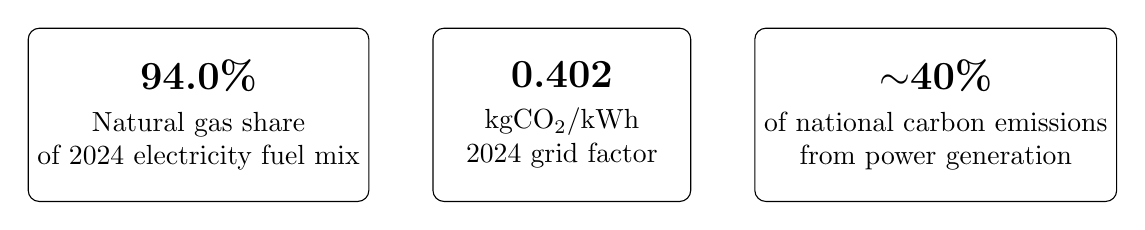
\begin{tikzpicture}[box/.style={draw,rounded corners,align=center,minimum width=0.27\linewidth,minimum height=22mm}]
\node[box] (a) {\Large\textbf{94.0\%}\\[1mm]Natural gas share\\of 2024 electricity fuel mix};
\node[box,right=8mm of a] (b) {\Large\textbf{0.402}\\[1mm]kgCO$_2$/kWh\\2024 grid factor};
\node[box,right=8mm of b] (c) {\Large\textbf{$\sim$40\%}\\[1mm]of national carbon emissions\\from power generation};
\end{tikzpicture}
\caption{Singapore energy context from Energy Market Authority (EMA) 2024 data~\cite{ema2024context,ema2024futurefund}. The panel is reconstructed from authoritative reported values stored in \texttt{data/external/ema\_singapore\_energy\_context\_2024.csv}; it is not a project-model result.}
\label{fig:singapore-context}
\end{figure}

Figure~\ref{fig:smr-explainer} introduces the hydrogen pathway at a deliberately simpler level than the detailed model. Feed carbon enters with natural gas. Reforming converts methane and steam to syngas; WGS converts CO and steam toward CO$_2$ and additional H$_2$; CO$_2$ separation removes a concentrated carbon stream; PSA produces high-purity hydrogen and a carbon-bearing tail gas. CCS changes where much of the carbon goes, but it does not remove the feedstock carbon from the chemistry~\cite{ieaghg2017smr}.


The nuclear proposal changes the \emph{heat source}, not the feed-carbon chemistry. Figure~\ref{fig:nuclear-heat-explainer} separates those ideas. A fired reformer supplies high-temperature heat by combustion; the nuclear-assisted concept instead transfers reactor heat through helium and an intermediate heat exchanger. The final design hierarchy is a 950$^\circ$C-class JAEA primary-helium hardware envelope $\rightarrow$ 900$^\circ$C delivered process heat $\rightarrow$ 871$^\circ$C reformer outlet. The specific INL Case-6 ROT is 925$^\circ$C~\cite{inltev961}, while JAEA/JAERI provides the 950$^\circ$C-class hardware precedent~\cite{jaeri2004gthtr300c}. Feedstock carbon still requires capture and lifecycle accounting.

\begin{figure}[htbp]
\centering
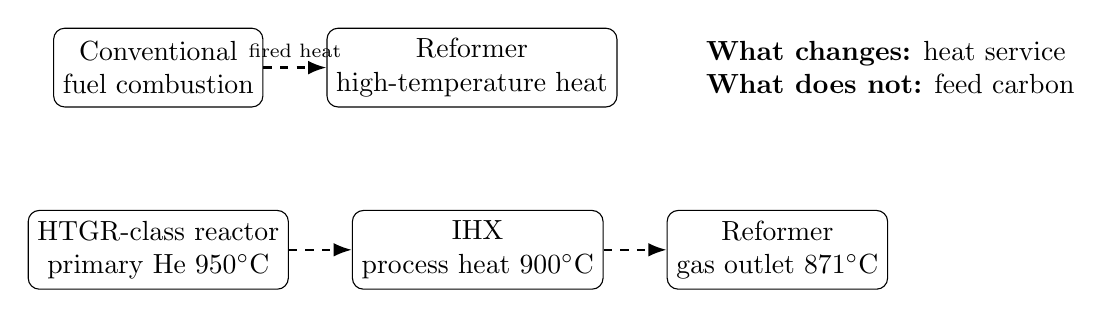
\begin{tikzpicture}[>=Latex,node distance=8mm,unit/.style={draw,rounded corners,align=center,minimum height=10mm,minimum width=25mm},arr/.style={->,thick},heat/.style={->,thick,dashed}]
\node[unit] (fire) {Conventional\\fuel combustion};
\node[unit,right=of fire] (r1) {Reformer\\high-temperature heat};
\draw[heat](fire)--node[above,font=\scriptsize]{fired heat}(r1);
\node[below=13mm of fire,unit] (reactor) {HTGR-class reactor\\primary He 950$^\circ$C};
\node[right=of reactor,unit] (ihx) {IHX\\process heat 900$^\circ$C};
\node[right=of ihx,unit] (r2) {Reformer\\gas outlet 871$^\circ$C};
\draw[heat](reactor)--(ihx);\draw[heat](ihx)--(r2);
\node[right=10mm of r1,align=left] {\textbf{What changes:} heat service\\\textbf{What does not:} feed carbon};
\end{tikzpicture}
\caption{Original two-layer explanation of nuclear assistance. The concept substitutes a high-temperature heat-delivery chain for fired reformer heat; it does not eliminate carbon entering as natural-gas feed. Temperatures show the final literature-supported design ladder; the 950$^\circ$C value is the JAEA hardware envelope and the 900/871$^\circ$C process pair is anchored to INL~\cite{inltev961,jaeri2004gthtr300c}.}
\label{fig:nuclear-heat-explainer}
\end{figure}


\subsection{Why an HTGR can supply process heat safely across an interface}
A high-temperature gas-cooled reactor (HTGR) uses helium as coolant. Helium is chemically inert and remains gaseous at reactor temperatures, making it suitable for carrying high-grade heat. HTGR fuel commonly uses coated particles (TRISO): the fuel kernel is surrounded by multiple ceramic/carbon barrier layers. For this project, the important point is not reactor-physics detail but the resulting engineering capability to operate with high-temperature helium~\cite{jaeahttr,jaeri2004gthtr300c}.

The intermediate heat exchanger (IHX) is the isolation boundary between the reactor primary circuit and the chemical heat-transfer circuit. Primary helium transfers heat across exchanger walls to a separate secondary-helium loop; the secondary helium then heats the reformer. Thus \textbf{reactor primary coolant does not enter the hydrogen process}.

\begin{figure}[htbp]\centering
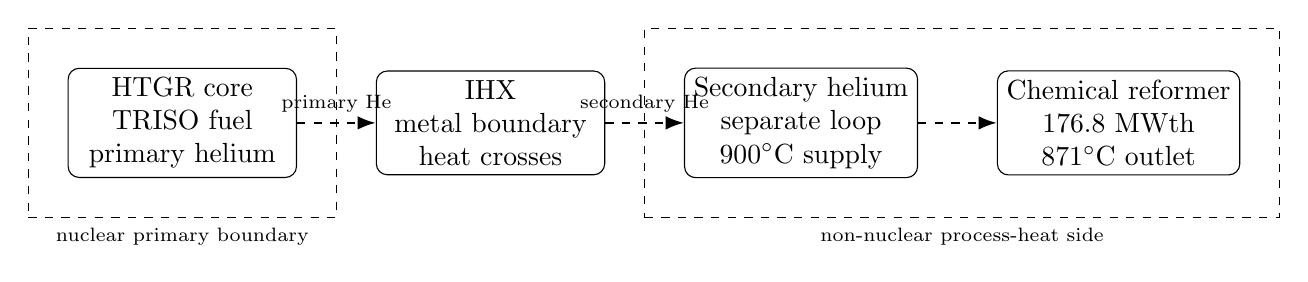
\begin{tikzpicture}[>=Latex,node distance=10mm,unit/.style={draw,rounded corners,align=center,minimum height=13mm,minimum width=29mm},arr/.style={->,thick},heat/.style={->,thick,dashed}]
\node[unit] (core) {HTGR core\\TRISO fuel\\primary helium};
\node[unit,right=of core] (ihx) {IHX\\metal boundary\\heat crosses};
\node[unit,right=of ihx] (sec) {Secondary helium\\separate loop\\900$^\circ$C supply};
\node[unit,right=of sec] (ref) {Chemical reformer\\176.8 MWth\\871$^\circ$C outlet};
\draw[heat](core)--node[above,font=\scriptsize]{primary He}(ihx);
\draw[heat](ihx)--node[above,font=\scriptsize]{secondary He}(sec);
\draw[heat](sec)--(ref);
\node[draw,dashed,fit=(core),inner sep=5mm,label=below:{\scriptsize nuclear primary boundary}] {};
\node[draw,dashed,fit=(sec)(ref),inner sep=5mm,label=below:{\scriptsize non-nuclear process-heat side}] {};
\end{tikzpicture}
\caption{Original isolation schematic reconstructed from HTGR/IHX architecture reported by JAEA/JAERI~\cite{jaeahttr,jaeri2004gthtr300c,nishihara2007potential}. It emphasizes the safety-relevant conceptual point: heat crosses the IHX, while the primary reactor coolant and chemical process remain separate circuits.}
\label{fig:ihx-isolation}
\end{figure}

The user-provided project-source diagrams were inspected as technical visual references during final QA. They contain useful depictions of fired reforming, amine capture, PSA, HTGR helium loops and IHX coupling, but their supplied filenames do not consistently describe their pictured systems. They were therefore not copied into the manuscript; the explanatory figures above were recreated from source-supported engineering concepts with primary-source attribution.

\section{System boundary and comparison basis}
The final candidate boundary follows the source INL process:
\[
\text{natural gas + steam}\rightarrow\text{SMR}\rightarrow\text{WGS}
\rightarrow\text{CO$_2$ capture}\rightarrow\text{PSA}\rightarrow\text{H$_2$}.
\]
High-temperature nuclear heat replaces reformer firing in the final Case-6 architecture. The lifecycle boundary adds upstream natural-gas supply, nuclear heat allocation, process electricity and CO$_2$ transport/storage. The economic boundary adds natural gas, full reactor cogeneration burden, incremental CCS capital, integration/site allowance and T\&S, with net exported electricity valued separately.

The principal baseline is INL's conventional no-capture SMR at the same 130 MMSCFD H$_2$ output~\cite{inltev953}. This provides a source-consistent direct-emissions and natural-gas comparison rather than scaling an unrelated plant. IEAGHG Case 1A remains an external conventional-SMR+CCS comparator, but its Singapore economics are not used to overwrite the final INL common-output baseline.

\section{Model formulation}\label{sec:model-formulation}

\subsection{Process model and literature inputs}
The model is literature-anchored rather than wholly first-principles. Its chemical-process basis is INL/NGNP Case 6. INL selected an 871$^\circ$C reformer outlet, steam/carbon ratio 3.0 and 88\% PSA recovery~\cite{inltev953}; TEV-961 reports that a 925$^\circ$C HTGR outlet supplies 900$^\circ$C process heat and the full 176.8 MWth reforming duty at that target~\cite{inltev961}. The source process produces 130 MMSCFD H$_2$ from 34.0 MMSCFD natural gas with 17.3 MWe process demand, 1,927 short ton/day captured CO$_2$ and 142 short ton/day emitted CO$_2$~\cite{inltev961}. The same INL model family provides the 130-MMSCFD conventional no-capture baseline: 52.5 MMSCFD natural gas and 3,205 short ton/day emitted CO$_2$~\cite{inltev953}.


\subsection{Model scope}
The operative calculation combines literature-derived process/reactor parameters, declared screening assumptions, engineering balances and derived Rust outputs. Earlier fixed-scale Gate-5 and Review-5 studies remain reproducible audit evidence in the repository but are not used as the final-design result.


\section{Nuclear-to-reformer heat integration}\label{sec:heat-integration}


The whole-system heat question is $\dot Q_{\mathrm{required}}\leq\dot Q_{\mathrm{available}}$, with both terms in MWth at compatible temperatures. This inequality checks capacity only; an actual heat exchanger must also maintain a positive temperature driving force throughout its length and satisfy material and transient limits.

\subsection{Temperature cascade and reformer heat requirement}
The first engineering question is physical: can the reactor supply enough heat, at a high enough temperature, to run the reformer? The reactor is therefore selected from the chemical-process requirement rather than the reverse. INL Case 6 reports a reformer outlet temperature $T_{\rm reformer}=871\,^{\circ}\mathrm C$, secondary-helium supply $T_{\rm He,supply}=900\,^{\circ}\mathrm C$, reactor outlet $T_{\rm reactor,out}=925\,^{\circ}\mathrm C$, and source process duty $\dot Q_{\rm process}=176.8$ MWth~\cite{inltev953,inltev961}.

To show the available temperature head between the reported secondary-helium supply location and reformer outlet, define
\begin{equation}\label{eq:reported-process-dt-general}
\Delta T_{\rm process,reported}
=T_{\rm He,supply}-T_{\rm reformer},
\end{equation}
where $\Delta T_{\rm process,reported}$ is the reported-location temperature difference (K), $T_{\rm He,supply}$ is secondary-helium supply temperature ($^{\circ}$C), and $T_{\rm reformer}$ is reformer outlet-gas temperature ($^{\circ}$C). Substitution of the cited source states gives
\begin{equation}\label{eq:reported-process-dt}
\Delta T_{\rm process,reported}
=900-871=29~\mathrm K.
\end{equation}
Equation~\ref{eq:reported-process-dt} is a reported-location difference, not a minimum local reformer pinch; local tube-wall, catalyst-bed and gas-temperature profiles are not all available.

The corresponding reported reactor-to-secondary-helium difference is
\begin{equation}\label{eq:ihx-dt-general}
\Delta T_{\rm IHX}
=T_{\rm reactor,out}-T_{\rm He,supply},
\end{equation}
where $\Delta T_{\rm IHX}$ is the reported primary-to-secondary outlet difference (K) and $T_{\rm reactor,out}$ is reactor outlet temperature ($^{\circ}$C). Using the INL Case-6 values~\cite{inltev961},
\begin{equation}\label{eq:temperature-cascade}
\Delta T_{\rm IHX}=925-900=25~\mathrm K.
\end{equation}
Thus the source temperature sequence is $925\rightarrow900\rightarrow871\,^{\circ}\mathrm C$; the 25 K and 29 K values are consequences of the reported source states rather than independently selected project pinch assumptions.

Finally, the source-reported 176.8 MWth process duty is checked against its secondary-helium states rather than re-derived from them. The steady sensible-heat relation is
\begin{equation}\label{eq:helium-heat-general}
\dot Q=\dot m_{\rm He}\,\bar c_{p,\rm He}
(T_{\rm in}-T_{\rm out}),
\end{equation}
where $\dot Q$ is thermal duty (kW), $\dot m_{\rm He}$ is secondary-helium mass flow (kg/s), $\bar c_{p,\rm He}$ is mean helium heat capacity (kJ kg$^{-1}$ K$^{-1}$), and $T_{\rm in}-T_{\rm out}$ is the helium temperature decrease (K). INL reports $\dot m_{\rm He}=78.49$ kg/s, $T_{\rm in}=900\,^{\circ}\mathrm C$ and $T_{\rm out}\approx466\,^{\circ}\mathrm C$~\cite{inltev961}. Solving Eq.~\ref{eq:helium-heat-general} for the implied mean heat capacity gives
\begin{equation}\label{eq:helium-cp-check}
\bar c_{p,\rm He}
=\frac{176.8\times10^3}
{78.49(900-466)}
\approx5.19~\mathrm{kJ\,kg^{-1}\,K^{-1}}.
\end{equation}
This is an independent consistency check on the source duty; it does not imply that the constant-$c_p$ equation generated INL's Aspen duty.

\subsection{Reactor selection from the process requirement}
Representative water-cooled SMRs provide useful electricity, steam, desalination and lower-temperature process heat, but their water-cooled outlet temperatures are far below the approximately 900$^\circ$C heating-medium requirement.  They therefore require a separate temperature-augmentation route for this direct-heat application.  This is an application-specific temperature mismatch, not a claim that LWRs are generally inferior.

HTTR passes the temperature filter: its 30 MWth reactor has demonstrated 950$^\circ$C operation~\cite{jaeahttr2026ops}.  It fails the project-scale filter because
\[
176.8/30=5.89,
\]
so HTTR is used as experimental evidence rather than as the project heat source.  HTR-PM provides valuable commercial HTGR operating, licensing and safety precedent, but its demonstrated plant is a steam-cycle architecture rather than the 900$^\circ$C secondary-helium reformer interface required here.  JAEA's GTHTR300C family, in contrast, is a 600 MWth process-heat/cogeneration design with 950$^\circ$C reactor-outlet and approximately 900$^\circ$C secondary-helium conditions~\cite{nishihara2007potential}.  It therefore passes the temperature, scale and process-heat-architecture filters.

The project is consequently described as a \textbf{GTHTR300C-class / GTHTR300C-informed screening architecture}, not as an exact GTHTR300C plant: the project uses the INL 925/900/871$^\circ$C operating point and 176.8 MWth duty rather than the exact JAEA heat split.

\begin{table}[htbp]\centering\scriptsize
\caption{Application-specific reactor evidence screen.  Dispositions are evidence categories, not technology rankings.}
\label{tab:reactor-screen}
\begin{tabular}{p{0.16\linewidth}p{0.15\linewidth}p{0.19\linewidth}p{0.23\linewidth}p{0.19\linewidth}}
\toprule
Candidate & Scale & Temperature evidence & Direct process-heat fit & Disposition\\ \midrule
Water-cooled SMR family & relevant modular scales & lower-temperature water/steam class & requires temperature augmentation for 900$^\circ$C heat & comparator; not direct-heat basis\\
HTTR & 30 MWth~\cite{jaeahttr2026ops} & 950$^\circ$C demonstrated~\cite{jaeahttr2026ops} & temperature yes; scale no & demonstrator/evidence\\
HTR-PM & operating multi-module HTGR & steam-cycle operating evidence & strong HTGR maturity; operating plant is not 900$^\circ$C secondary-He SMR & safety/licensing comparator\\
GTHTR300C & 600 MWth design~\cite{nishihara2007potential} & 950$^\circ$C reactor / 900$^\circ$C secondary He~\cite{nishihara2007potential} & explicit hydrogen/process-heat architecture~\cite{nishihara2007potential} & retained design basis, conditional\\
Case-6 benchmark & 600 MWth class (source basis above) & 925$\rightarrow$900$\rightarrow$871$^\circ$C~\cite{inltev953,inltev961} & 176.8 MWth source-model duty~\cite{inltev961} & GTHTR300C-informed screen\\
\bottomrule
\end{tabular}
\end{table}

\subsection{Reactor capacity, IHX scale and helium-loop check}
The following labelled one-train fractions and 423.2 MWth identity reproduce the original Case-6 benchmark; they are retained for auditability, not as the preferred final thermal allocation. The preferred architecture doubles the chemical process duty to 353.6 MWth, uses 95.6\% of the rounded 370 MWth process branch, and leaves a conditional 246.4 MWth full-power residual (Section~\ref{sec:energy-performance}). Neither residual is a cooling-duty estimate.
INL supplies the chemical-process duty; Nishihara et al. supplies the selected GTHTR300C hardware/economic architecture. They are deliberately kept as separate evidence layers.

The selected source architecture is a 600 MWth GTHTR300C-class design~\cite{nishihara2007potential}. JAEA's high-hydrogen variant provides approximately 371 MWth of process-heat branch capability (rounded to 370 MWth in the canonical economic model) and approximately 87--88 MWe of complementary source electricity~\cite{nishihara2007potential}. The 370 MWth value is a source process-heat branch/economic architecture, not the rating of one physical IHX.

To quantify how much of the selected reactor rating is required by the INL process, define
\begin{equation}\label{eq:reactor-process-fraction}
f_{\rm process}=\frac{\dot Q_{\rm process}}{\dot Q_{\rm reactor}},
\end{equation}
where $f_{\rm process}$ is the reactor thermal-capacity fraction allocated to process heat (-), $\dot Q_{\rm process}$ is the source process duty (MWth), and $\dot Q_{\rm reactor}$ is reactor thermal rating (MWth). Using 176.8 MWth from INL~\cite{inltev961} and 600 MWth from Nishihara~\cite{nishihara2007potential},
\begin{equation}\label{eq:reactor-process-fraction-sub}
f_{\rm process}=\frac{176.8}{600}=0.2947\approx29.5\%.
\end{equation}
The derived 29.5\% is an aggregate reactor-capacity fraction, not a component qualification result.

The remaining thermal capacity under this simple accounting is
\begin{equation}\label{eq:remaining-thermal}
\dot Q_{\rm remaining}=\dot Q_{\rm reactor}-\dot Q_{\rm process}
=600-176.8=423.2~\mathrm{MW_{th}}.
\end{equation}
Here $\dot Q_{\rm remaining}$ is unallocated reactor thermal capacity (MWth). It is not automatically electricity output, cooling duty, turbine input or waste heat because no validated project off-design power-cycle/internal-load model is available.

The process duty also occupies
\begin{equation}\label{eq:branch-utilisation}
f_{\rm branch}=\frac{176.8}{370}=0.478\approx47.8\%
\end{equation}
of the rounded source high-hydrogen heat branch, leaving 193.2 MWth nominal branch margin. Here $f_{\rm branch}$ is only an architecture-level utilisation fraction; the cited 370 MWth branch~\cite{nishihara2007potential} is not one exchanger rating.

Component scale is checked separately. The JAERI GTHTR300C design report provides an approximately 170 MWth reference physical IHX~\cite{jaeri2004gthtr300c}, whereas INL requires 176.8 MWth~\cite{inltev961}. Therefore
\begin{equation}\label{eq:ihx-duty-gap}
\Delta \dot Q_{\rm IHX}=176.8~\mathrm{MW_{th}}-170~\mathrm{MW_{th}}=6.8~\mathrm{MW_{th}},
\end{equation}
and
\begin{equation}\label{eq:ihx-duty-ratio}
R_{\rm IHX}=\frac{176.8~\mathrm{MW_{th}}}{170~\mathrm{MW_{th}}}=1.040.
\end{equation}
$\Delta\dot Q_{\rm IHX}$ is the project-minus-reference duty (MWth) and $R_{\rm IHX}$ is their dimensionless ratio. The project duty is thus about 4.0\% above the single reference-IHX duty; a larger, parallel or redesigned exchanger remains a qualification requirement.

For the process-side helium screen, INL Case 6 provides approximately 900$^\circ$C supply, 466$^\circ$C return and 78.49 kg/s~\cite{inltev961}. Using project screening parameter R-08, an average $c_p=5.2$ kJ kg$^{-1}$ K$^{-1}$ selected only to check consistency with the source flow, gives
\begin{equation}\label{eq:helium-flow-check}
\dot m_{He}=\frac{176.8\times10^3}{5.2(900-466)}\approx78.34\ {\rm kg/s},
\end{equation}
which is used only as a constant-$c_p$ verification screen~\cite{inltev961}.

\input{../results/final_design/generated/heat_flow_figure.tex}



\section{Hydrogen production and material balance}\label{sec:hydrogen}
The thermal calculation establishes that the proposed heat path is large enough at screening level; the next question is what hydrogen service that heat supports. The chemical-process model is not re-solved from first principles in this project. Instead, INL Case 6 supplies the source-model process result: 130 MMSCFD H$_2$, an 871$^\circ$C reformer outlet, steam/carbon ratio 3.0 and 88\% PSA hydrogen recovery~\cite{inltev953,inltev961}.

The chemistry explains the sequence represented by that source model. Steam methane reforming converts methane and steam toward carbon monoxide and hydrogen,
\[
\mathrm{CH_4+H_2O\rightleftharpoons CO+3H_2},
\]
and the Water-Gas Shift reaction converts carbon monoxide and steam toward carbon dioxide and additional hydrogen,
\[
\mathrm{CO+H_2O\rightleftharpoons CO_2+H_2}.
\]
Carbon dioxide is then separated before Pressure Swing Adsorption (PSA) recovers hydrogen from the remaining gas. The reported 88\% value is \emph{hydrogen recovery}, not hydrogen purity.

INL also reports an instantaneous hydrogen mass rate of approximately 29,000 lb/h for the common service~\cite{inltev953,inltev961}. The annualisation below converts that source rate to annual production using the declared 85\% availability. This distinction matters: 130 MMSCFD and 29,000 lb/h are \textbf{source-model outputs}; approximately 97,946 t/y is the project's \textbf{derived annual result}.


\subsection{Annual hydrogen production from the source rate}
INL reports the common hydrogen service as 130 MMSCFD and approximately 29,000 lb/h~\cite{inltev953,inltev961}. Using Assumption A-02, $A=0.85$~\cite{nishihara2007potential}, annual hydrogen production is calculated from
\begin{equation}\label{eq:annual-h2-general}
M_{H_2}=\dot m_{H_2}\,t_{\rm year}\,A,
\end{equation}
where $M_{H_2}$ is annual hydrogen production (t/y), $\dot m_{H_2}$ is instantaneous hydrogen mass rate (t/h), $t_{\rm year}=8760$ h/y, and $A$ is annual availability (-). Converting the cited 29,000 lb/h source rate gives
\begin{equation}\label{eq:annual-h2}
M_{H_2}=29{,}000\frac{\mathrm{lb}}{\mathrm h}
\left(0.45359237\frac{\mathrm{kg}}{\mathrm{lb}}\right)
(8760\,\mathrm{h/y})(0.85)
\left(\frac{1\,\mathrm t}{1000\,\mathrm{kg}}\right)
=97{,}946~\mathrm{t/y}.
\end{equation}
This is a project annualisation of the source instantaneous rate, not a separate literature-reported annual plant output.


\section{Carbon balance and CCS}\label{sec:carbon}
\subsection{Lifecycle-model boundary and formulation}
Once the heat balance closes, the analysis follows the carbon. Source direct emissions are annualized at the selected mature-design 85\% availability. Lifecycle accounting adds the difference in upstream natural-gas burden and subtracts nuclear-heat, incremental auxiliary-electricity and CO$_2$ transport/storage burdens. The upstream-gas factor is a global International Energy Agency (IEA) proxy~\cite{iea2026lng}; the nuclear lifecycle proxy is from the United Nations Economic Commission for Europe (UNECE) and is global rather than Singapore-specific~\cite{unece2022lca}. The CCS transport burden remains an explicit screening assumption.



\subsection{Carbon balance and lifecycle emissions}
The source process reports 3,205 short ton/day baseline emissions~\cite{inltev953}, and 142 short ton/day residual emissions plus 1,927 short ton/day captured CO$_2$ for Case 6~\cite{inltev961}. These source values are converted rather than reverse-engineered from an assumed pure-methane feed, because the INL process model already distinguishes feed, fuel and process streams. The annualisation uses the Nishihara design-study availability $A=0.85$ (Assumption A-02)~\cite{nishihara2007potential}. Using the standard conversion 1 short ton = 0.90718474 t, the general annualization for a source daily CO$_2$ rate $\dot M_{CO_2,d}$ is
\begin{equation}\label{eq:co2-annual-general}
M_{CO_2,y}=\dot M_{CO_2,d}(0.90718474)(365)A,
\end{equation}
where $M_{CO_2,y}$ is annual CO$_2$ mass (t/y), $\dot M_{CO_2,d}$ is source CO$_2$ rate (short ton/d), and $A$ is availability (-). For the baseline:
\begin{equation}\label{eq:base-direct}
E_{\rm base,direct}=3205\frac{\mathrm{short\ ton}}{\mathrm d}
(0.90718474)\frac{\mathrm t}{\mathrm{short\ ton}}(365)(0.85)
=902{,}060~\mathrm{t/y}.
\end{equation}
\begin{equation}\label{eq:cand-direct}
E_{\rm cand,direct}=142(0.90718474)(365)(0.85)
=39{,}966~\mathrm{t/y}.
\end{equation}
so
\begin{equation}\label{eq:direct-avoided}
A_{\rm direct}=902{,}060-39{,}966=862{,}094~\mathrm{tCO_2/y}.
\end{equation}
The same conversion gives
\begin{equation}\label{eq:captured-annual}
M_{\rm captured}=1927(0.90718474)(365)(0.85)
=542{,}362~\mathrm{tCO_2/y}.
\end{equation}

Natural-gas use falls from 52.5 MMSCFD~\cite{inltev953} to 34.0 MMSCFD~\cite{inltev961}. To convert a volumetric gas rate $F_{\rm NG}$ (MMSCFD) to daily energy, the screening model uses
\begin{equation}\label{eq:ng-energy}
Q_{\rm NG,d}=F_{\rm NG}(10^6)(HHV_{\rm NG})(1.05505585262\times10^{-6}),
\end{equation}
where $Q_{\rm NG,d}$ is natural-gas energy (GJ/d), $HHV_{\rm NG}$ is gas higher heating value (Btu/scf), and the final factor is GJ/Btu. Assumption A-03 uses $HHV_{\rm NG}=1044$ Btu/scf as the project screening basis; it is not asserted as an INL-measured gas property. Assumption A-04 uses the IEA global-average 11.5 kgCO$_2$e/GJ gas-supply factor~\cite{iea2026lng}. Annual upstream emissions are calculated as
\begin{equation}\label{eq:upstream-ng}
E_{\rm NG,up}=Q_{\rm NG,d}(365)A\,e_{\rm NG}/1000,
\end{equation}
where $E_{\rm NG,up}$ is upstream emissions (tCO$_2$e/y) and $e_{\rm NG}=11.5$ kgCO$_2$e/GJ is Assumption A-04~\cite{iea2026lng}. For the 52.5 MMSCFD baseline~\cite{inltev953},
\begin{equation}\label{eq:upstream-ng-base}
\begin{aligned}
E_{\rm NG,up,base}
&=\left[(52.5~\mathrm{MMSCFD})(10^6~\mathrm{scf/MMSCF})(1044~\mathrm{Btu/scf})\right.\\
&\qquad\left.\times(1.05505585262\times10^{-6}~\mathrm{GJ/Btu})\right]
(365~\mathrm{d/y})(0.85)
\frac{11.5~\mathrm{kgCO_2e/GJ}}{1000~\mathrm{kg/t}}\\
&\approx206{,}322~\mathrm{tCO_2e/y}.
\end{aligned}
\end{equation}
Here 1044 Btu/scf is Assumption A-03 and 11.5 kgCO$_2$e/GJ is the IEA global proxy (A-04)~\cite{iea2026lng}. For the 34.0 MMSCFD candidate~\cite{inltev961},
\begin{equation}\label{eq:upstream-ng-candidate}
\begin{aligned}
E_{\rm NG,up,cand}
&=\left[(34.0~\mathrm{MMSCFD})(10^6~\mathrm{scf/MMSCF})(1044~\mathrm{Btu/scf})\right.\\
&\qquad\left.\times(1.05505585262\times10^{-6}~\mathrm{GJ/Btu})\right]
(365~\mathrm{d/y})(0.85)
\frac{11.5~\mathrm{kgCO_2e/GJ}}{1000~\mathrm{kg/t}}\\
&\approx133{,}618~\mathrm{tCO_2e/y}.
\end{aligned}
\end{equation}
The upstream saving used in the lifecycle ledger is therefore
\begin{equation}\label{eq:upstream-ng-saving}
A_{\rm upstream}=E_{\rm NG,up,base}-E_{\rm NG,up,cand}
=206{,}322-133{,}618\approx72{,}704~\mathrm{tCO_2e/y}.
\end{equation}
$E_{\rm NG,up,base}$ and $E_{\rm NG,up,cand}$ are annual upstream gas-supply emissions (tCO$_2$e/y), and $A_{\rm upstream}$ is their project-derived difference (tCO$_2$e/y).  The new candidate burdens use Assumption A-05, the UNECE 5.5 kgCO$_2$e/MWh$_e$ nuclear-electricity lifecycle anchor~\cite{unece2022lca}. For direct heat, Assumption A-06 multiplies that electricity factor by the declared 0.504 MWh$_e$-equivalent/MWh$_{th}$ allocation proxy; this is not a published direct-heat LCA. The auxiliary term uses the source 17.3 MWe candidate demand~\cite{inltev961} minus Assumption A-01 = 6.3 MWe, a retained historical project screening anchor rather than an INL common-output value. Assumption A-07 = 0.025 tCO$_2$e/tCO$_2$ is likewise a generic project T\&S lifecycle screen, not a Singapore-route measurement. Thus the nuclear-heat lifecycle burden is calculated from
\begin{equation}\label{eq:nuclear-lca-general}
E_{\rm nuclear}=\dot Q_{\rm process}(1000)t_{\rm op}(e_{\rm nuc}\eta_e)/10^6,
\end{equation}
where $\dot Q_{\rm process}$ is process heat (MWth), $t_{\rm op}$ is operating time (h/y), $e_{\rm nuc}$ is the nuclear electricity lifecycle anchor (kgCO$_2$e/MWh$_e$), and $\eta_e=0.504$ is the declared allocation factor. Numerically,
\begin{equation}\label{eq:nuclear-lca}
E_{\rm nuclear}=176.8(1000)(7446)(5.5\times0.504)/10^6
=3{,}649~\mathrm{tCO_2e/y},
\end{equation}
The incremental auxiliary burden is
\begin{equation}\label{eq:aux-lca-general}
E_{\rm aux}=(P_{\rm cand}-P_{\rm common})(1000)t_{\rm op}e_{\rm nuc}/10^6,
\end{equation}
where $P_{\rm cand}$ and $P_{\rm common}$ are candidate and retained common electricity demands (MWe). Substitution gives
\begin{equation}\label{eq:aux-lca}
E_{\rm aux}=(17.3-6.3)(1000)(7446)(5.5)/10^6
=450~\mathrm{tCO_2e/y},
\end{equation}
and the T\&S lifecycle screen is
\begin{equation}\label{eq:ts-lca-general}
E_{\rm T\&S}=e_{\rm T\&S}M_{\rm captured},
\end{equation}
where $e_{\rm T\&S}$ is the screening T\&S factor (tCO$_2$e/tCO$_2$) and $M_{\rm captured}$ is captured CO$_2$ (t/y). Thus
\begin{equation}\label{eq:ts-lca}
E_{\rm T\&S}=0.025(542{,}362)=13{,}559~\mathrm{tCO_2e/y}.
\end{equation}
Direct CO$_2$ and lifecycle CO$_2$e are not interchangeable. The conventional and candidate plant stacks first determine the direct saving in Eq.~\ref{eq:direct-avoided}. Lifecycle accounting then adds the upstream saving from Eq.~\ref{eq:upstream-ng-saving} and subtracts the nuclear, auxiliary-electricity and T\&S burdens from Eqs.~\ref{eq:nuclear-lca}, \ref{eq:aux-lca} and \ref{eq:ts-lca}:
\begin{equation}\label{eq:lifecycle-avoided}
A_{\rm lifecycle}=A_{\rm direct}+A_{\rm upstream}-E_{\rm nuclear}-E_{\rm aux}-E_{\rm T\&S}.
\end{equation}

\begin{table}[htbp]\centering\scriptsize
\caption{Canonical lifecycle-emissions ledger generated by Rust. SAVED means less than the conventional baseline; ADDED means a new candidate burden.}
\label{tab:co2-ledger}
\pgfplotstabletypeset[col sep=comma,
columns={item,direction,change_tco2e_y,meaning},
columns/item/.style={string type,column name=Item,column type={p{0.31\linewidth}}},
columns/direction/.style={string type,column name=Direction,column type={p{0.11\linewidth}}},
columns/change_tco2e_y/.style={fixed,precision=0,column name={tCO$_2$e/y},column type=r},
columns/meaning/.style={string type,column name=Meaning,column type={p{0.31\linewidth}}},
every head row/.style={before row=\toprule,after row=\midrule},
every last row/.style={after row=\bottomrule}]
{../results/final_design/generated/lifecycle_ledger.csv}
\end{table}

\begin{figure}[htbp]\centering
\input{../results/final_design/generated/co2_bridge_figure.tex}
\caption{Rust-generated lifecycle contribution bridge.  Positive bars are savings; negative bars are candidate lifecycle burdens.  The net bar reproduces the canonical lifecycle result.}
\label{fig:co2-bridge}
\end{figure}

Using Eq.~\ref{eq:lifecycle-avoided}, the arithmetic reconciliation is
\begin{equation}\label{eq:lifecycle-reconciliation}
862{,}093.8+72{,}703.8-3{,}649.2-450.5-13{,}559.0
=\mathbf{917{,}138.9~tCO_2e/y}.
\end{equation}
The candidate lifecycle total is
\begin{equation}\label{eq:candidate-lifecycle-total}
E_{\rm cand,LC}=39{,}966.48+133{,}617.86+3{,}649.21+450.48+13{,}559.05
=191{,}243.07~\mathrm{tCO_2e/y}.
\end{equation}
Using annual hydrogen production from Eq.~\ref{eq:annual-h2}, the candidate lifecycle intensity is
\begin{equation}\label{eq:lifecycle-intensity}
I_{H_2}=\frac{E_{\rm cand,LC}}{M_{H_2}}
=\frac{191{,}243.07~\mathrm{tCO_2e/y}}{97{,}946.0~\mathrm{tH_2/y}}
\approx1.95~\mathrm{kgCO_2e/kgH_2}.
\end{equation}
Here $E_{\rm cand,LC}$ is candidate lifecycle emissions (tCO$_2$e/y), $M_{H_2}$ is annual hydrogen mass (t/y), and $I_{H_2}$ is lifecycle carbon intensity; t/t is numerically identical to kg/kg.

Lifecycle avoidance exceeds direct avoidance because the approximately 72.7 ktCO$_2$e/y upstream natural-gas saving is larger than the approximately 17.7 ktCO$_2$e/y of new lifecycle burdens. Captured CO$_2$ is not added again to the numerator, avoiding double counting.  The one-tonne-scale difference obtained by adding rounded table entries is rounding only.

The lifecycle abatement result remains dominated by the same-output direct-emissions difference and lower natural-gas use. Cross-border CCS availability, mature-design reactor economics, the direct-heat lifecycle proxy and detailed reactor/process integration remain important screening limitations.

\section{Energy performance}\label{sec:energy-performance}
The supported energy result is a thermal allocation rather than a complete exergy or power-cycle analysis. The selected reactor design basis is 600 MWth, while the INL reformer duty is 176.8 MWth. Equation~\ref{eq:remaining-thermal} therefore leaves 423.2 MWth of unallocated reactor thermal capacity. This value is not electricity output, turbine input, cooling duty or waste heat because the current model does not contain a validated off-design power-cycle and internal-load calculation.

The corresponding source-architecture checks remain in Section~\ref{sec:heat-integration}: the project duty is within the approximately 370/371 MWth source process-heat branch, while physical-IHX qualification is assessed separately against the approximately 170 MWth reference exchanger. No exergy analysis is claimed.

\section{Techno-economic analysis}\label{sec:tea}
\subsection{Economic-model boundary and formulation}
After the carbon ledger establishes the denominator for abatement cost, the economic model constructs the numerator. The principal mature case uses the coherent Nishihara reference economics: 59.7 billion JPY plant cost, 0.52 JPY/MJ heat and 4.9 JPY/kWh electricity at 85\% availability~\cite{nishihara2007potential}. Because no validated project off-design electricity output is claimed, the controlling economic test assigns \textbf{S\$0/MWh electricity export value}. To avoid free reactor capacity, the calculation charges the full published source-product burden: the source 370 MWth heat product at its source heat cost plus the source 88 MWe generation at its source electricity cost. This is a conservative economic allocation, not a claim that the project itself exports 88 MWe.

The source's 70.9 billion JPY / 0.57 JPY/MJ / 5.5 JPY/kWh case is retained only as an adverse \emph{cost} sensitivity in which assigned IHX/secondary-loop cost doubles; it is not interpreted as increased exchanger capacity. CCS capital is anchored to IEAGHG Case 1A and T\&S remains a Singapore screening scenario~\cite{ieaghg2017smr,mticcs2025cost}.

Forward abatement cost remains
\begin{equation}\label{eq:abatement-cost-definition}
C_{\rm abatement}=\frac{C_{\rm candidate}-C_{\rm baseline}}{A_{\rm avoided}}.
\end{equation}
where $C_{\rm candidate}$ and $C_{\rm baseline}$ are annual candidate and baseline costs (S\$/y), $A_{\rm avoided}$ is annual lifecycle abatement (tCO$_2$e/y), and $C_{\rm abatement}$ is forward abatement cost (S\$/tCO$_2$e). Section~\ref{sec:ledgers} provides the numerical substitution.



\subsection{Historical one-train differential screen (superseded)}
The following cost bridge is retained for numerical provenance, not as the controlling CN4252 economic answer. It predates the stronger E1 full-burden accounting and the E2B two-train maturation model. Its S\$3.725/t result must not be interpreted as a deployable FOAK price.\n\n\subsection{Techno-economic calculation}
The natural-gas saving is directly reproducible from the same cited 52.5 and 34.0 MMSCFD source rates. Assumption A-08 sets the gas price $P_{\rm NG}$ to S\$15/GJ as a project screening value, not a contracted Singapore tariff. Annual gas expenditure is
\begin{equation}\label{eq:ng-cost-general}
C_{\rm NG}=Q_{\rm NG,d}(365)A P_{\rm NG},
\end{equation}
where $C_{\rm NG}$ is annual gas cost (S\$/y). For the cited baseline flow~\cite{inltev953},
\begin{equation}\label{eq:ng-cost-base}
C_{\rm NG,base}
=\left[(52.5)(10^6)(1044)(1.05505585262\times10^{-6})\right]
(365)(0.85)(15)
\approx\mathrm{S\$}269.115~\mathrm{million/y},
\end{equation}
where the bracketed term is GJ/d and Assumption A-08 is $P_{\rm NG}=\mathrm{S\$}15$/GJ. For the cited candidate flow~\cite{inltev961},
\begin{equation}\label{eq:ng-cost-candidate}
C_{\rm NG,cand}
=\left[(34.0)(10^6)(1044)(1.05505585262\times10^{-6})\right]
(365)(0.85)(15)
\approx\mathrm{S\$}174.284~\mathrm{million/y}.
\end{equation}
The factors have dimensions MMSCFD$\times$scf/MMSCF$\times$Btu/scf$\times$GJ/Btu$\times$d/y$\times$S\$/GJ, leaving S\$/y.
hence
\begin{equation}\label{eq:ng-saving}
S_{\rm NG}=269.115-174.284
=\mathbf{S\$94.831~million/y}.
\end{equation}

The selected source economic burden is deliberately charged in full. Nishihara reports source heat cost $p_{h,0}=0.52$ JPY/MJ and source electricity cost $p_{e,0}=4.9$ JPY/kWh~\cite{nishihara2007potential}. Let $D_{JP}=112.27/99.59=1.12732$ be the recorded 2007-to-2025 Japan GDP-deflator factor (-) and $X_{JPY}=0.008117$ SGD/JPY the dated project FX conversion. The normalized heat price is
\begin{equation}\label{eq:heat-price-normalization}
\begin{aligned}
p_h&=p_{h,0}D_{JP}X_{JPY}(1000~\mathrm{MJ/GJ})\\
&=(0.52~\mathrm{JPY/MJ})(1.12732)(0.008117~\mathrm{SGD/JPY})\\
&\qquad\times(1000~\mathrm{MJ/GJ})
\approx\mathrm{S\$}4.758/\mathrm{GJ}.
\end{aligned}
\end{equation}
Similarly,
\begin{equation}\label{eq:electric-price-normalization}
\begin{aligned}
p_e&=p_{e,0}D_{JP}X_{JPY}(1000~\mathrm{kWh/MWh})\\
&=(4.9~\mathrm{JPY/kWh})(1.12732)(0.008117~\mathrm{SGD/JPY})\\
&\qquad\times(1000~\mathrm{kWh/MWh})
\approx\mathrm{S\$}44.837/\mathrm{MWh}.
\end{aligned}
\end{equation}
Here $p_h$ and $p_e$ are normalized source-product prices. The deflator and FX bases are documented project normalization inputs; the GDP deflator is a broad screening index, not a nuclear-construction index. Therefore
\begin{equation}\label{eq:source-heat-cost}
C_{\rm source,heat}
=(370~\mathrm{MW_{th}})(7446~\mathrm{h/y})(3.6~\mathrm{GJ/MWh})(4.758~\mathrm{S\$/GJ})
\approx\mathrm{S\$}47.193~\mathrm{million/y}.
\end{equation}
The 370 MWth source process-heat/economic branch is from Nishihara~\cite{nishihara2007potential}; 7446 h/y is $8760\times0.85$ using Assumption A-02; 3.6 GJ/MWh is an exact energy conversion; and 4.758 S\$/GJ is Eq.~\ref{eq:heat-price-normalization}. The dimensions reduce as MW$\times$h/y$\times$GJ/MWh$\times$S\$/GJ = S\$/y. This is the heat-product share of the selected published source economic burden.
\begin{equation}\label{eq:source-electric-cost}
C_{\rm source,electric}
=(88~\mathrm{MWe})(7446~\mathrm{h/y})(44.837~\mathrm{S\$/MWh})
\approx\mathrm{S\$}29.380~\mathrm{million/y}.
\end{equation}
The 88 MWe complementary source product is the rounded Nishihara high-hydrogen economic configuration~\cite{nishihara2007potential}; 44.837 S\$/MWh is Eq.~\ref{eq:electric-price-normalization}. MW$\times$h/y$\times$S\$/MWh reduces to S\$/y.
and
\begin{equation}\label{eq:source-total-cost}
C_{\rm source}\approx\mathbf{S\$76.572~million/y}.
\end{equation}
The 88 MWe term is used only to recover the full published source economic burden; it is not a project export claim.

IEAGHG Case 1A provides the source capture-capital anchor $C_{\rm CCS,0}=\mathrm{EUR}\,41.02$ million (2014 basis)~\cite{ieaghg2017smr}. The canonical reference capture scale is $M_0=387{,}805.2$ t/y and the project capture scale is $M_{\rm captured}=542{,}361.98$ t/y from Eq.~\ref{eq:captured-annual}. The project assumes linear captured-tonne scaling, exponent $\alpha=1$, together with the recorded 2014-to-2025 deflator proxy $D_{EU}=123.84/90.46=1.36834$ and dated FX $X_{EUR}=1.452$ SGD/EUR. Thus
\begin{equation}\label{eq:ccs-capex-general}
C_{\rm CCS}=C_{\rm CCS,0}D_{EU}X_{EUR}
\left(\frac{M_{\rm captured}}{M_0}\right)^{\alpha},
\end{equation}
where $C_{\rm CCS}$ is project screening capture CAPEX (S\$), $C_{\rm CCS,0}$ is source CAPEX (EUR), $D_{EU}$ is the price-year factor (-), $X_{EUR}$ is FX (SGD/EUR), and $\alpha=1$ is the explicit project scaling assumption. Numerically,
\begin{equation}\label{eq:ccs-capex-substitution}
C_{\rm CCS}
=(41.02~\mathrm{million~EUR})(1.36834)(1.452~\mathrm{SGD/EUR})
\left(\frac{542{,}361.98~\mathrm{t/y}}{387{,}805.2~\mathrm{t/y}}\right)
\approx\mathrm{S\$}114.036~\mathrm{million}.
\end{equation}
IEAGHG did not report S\$114.036 million for this project; it is the project-normalized, linearly scaled result. Capital is annualized using
\begin{equation}\label{eq:crf}
\mathrm{CRF}(i,n)=\frac{i(1+i)^n}{(1+i)^n-1},
\end{equation}
where $i$ is annual discount rate (-) and $n$ is economic life (y). Assumption A-13 retains the IEAGHG $i=0.08$ and $n=25$ y basis~\cite{ieaghg2017smr}; therefore
\begin{equation}\label{eq:ccs-annual-cost}
C_{\rm CCS,annual}=C_{\rm CCS}\,\mathrm{CRF}(0.08,25)
=(114.036~\mathrm{million~S\$})(0.09368)
\approx\mathbf{S\$10.683~million/y}.
\end{equation}
$C_{\rm CCS,annual}$ is annualized capture capital (S\$/y), and $\mathrm{CRF}(0.08,25)\approx0.09368$ y$^{-1}$.
Assumption A-14 is an explicit 10\% project integration/site capital allowance rather than an observed Singapore cost. The S\$546.283 million reactor/source capital basis is the normalized 59.7 billion JPY Nishihara source plant cost~\cite{nishihara2007potential}; S\$114.036 million is the project CCS CAPEX from Eq.~\ref{eq:ccs-capex-substitution}. Assumption A-15 applies the retained 3\% annualisation rate and 40-y life to this allowance; these are screening/design-study bases, not a financing offer. It contributes approximately
\begin{equation}\label{eq:integration-cost}
C_{\rm integration}=0.10(546.283+114.036)\,\mathrm{million}\,\mathrm{CRF}(0.03,40)\approx\mathbf{S\$2.857~million/y}.
\end{equation}
while Assumption A-16 sets T\&S to S\$15/tCO$_2$ as a project screening tariff, not an observed or contracted Singapore tariff. Official Singapore evidence is cited only for the separate statement that actual cross-border CCS costs remain unresolved~\cite{mticcs2025cost}. Using $M_{\rm captured}=542{,}362$ t/y from Eq.~\ref{eq:captured-annual},
\begin{equation}\label{eq:ts-cost}
C_{\rm T\&S}=542{,}362(15)
\approx\mathbf{S\$8.135~million/y}.
\end{equation}
Assumption A-17 sets project electricity revenue to exactly \textbf{S\$0/y} because no validated off-design export model exists; this is a conservative model boundary, not a market-price claim.
The economic ledger follows the same logic. The conventional baseline's natural-gas expenditure is replaced by lower candidate gas use plus the full selected source reactor economic burden, CCS annualisation, integration allowance and T\&S. Project electricity revenue is exactly zero.

\begin{table}[htbp]\centering\scriptsize
\caption{Canonical annual-cost ledger generated by Rust for the zero-electricity-credit model boundary.}
\label{tab:cost-ledger}
\pgfplotstabletypeset[col sep=comma,
columns={item,direction,annual_sgd,meaning},
columns/item/.style={string type,column name=Item,column type={p{0.31\linewidth}}},
columns/direction/.style={string type,column name=Direction,column type={p{0.11\linewidth}}},
columns/annual_sgd/.style={fixed,precision=0,column name={S\$/y},column type=r},
columns/meaning/.style={string type,column name=Meaning,column type={p{0.31\linewidth}}},
every head row/.style={before row=\toprule,after row=\midrule},
every last row/.style={after row=\bottomrule}]
{../results/final_design/generated/cost_ledger.csv}
\end{table}

Total money saved is approximately S\$94.831 million/y.  Total new represented costs are approximately S\$98.247 million/y, so
\begin{equation}\label{eq:annual-incremental-cost}
\Delta C_{\rm annual}
\approx98.247-94.831
=\mathbf{S\$3.416~million/y}.
\end{equation}
The final division is therefore
\begin{equation}\label{eq:abatement-cost-final}
C_{\rm abatement}
=\frac{\Delta C_{\rm annual}}{A_{\rm lifecycle}}
\approx\frac{\mathrm{S\$}3.416\ \mathrm{million/y}}{917{,}139\ \mathrm{tCO_2e/y}}
\approx\mathbf{S\$3.725/\mathrm{tCO_2e}}.
\end{equation}

\begin{figure}[htbp]\centering
\input{../results/final_design/generated/cost_bridge_figure.tex}
\caption{Rust-generated annual cost-contribution bridge.  Natural-gas savings are negative cost; reactor, CCS, integration and transport/storage are added costs.  Electricity revenue is zero by model boundary.}
\label{fig:cost-bridge}
\end{figure}




For the preferred mature case, the represented annual ledger is
\[
C_{\rm base,annual}=538.230~\mathrm{S\$\,million/y},\qquad
C_{\rm cand,annual}=616.814~\mathrm{S\$\,million/y},
\]
so that
\[
\Delta C_{\rm annual}
=C_{\rm cand,annual}-C_{\rm base,annual}
\approx78.583~\mathrm{S\$\,million/y}.
\]
The candidate ledger contains the normalized/annualized mature nuclear burden (S\$207.763 million/y), two-train integration/IHX allowance (S\$22.846 million/y), candidate NG, CCS and T\&S terms; the baseline ledger contains the corresponding two-train conventional NG/process cost basis. The project NG assumption remains S\$15/GJ and T\&S remains S\$15/t captured CO$_2$; neither is a contracted tariff. With E2B lifecycle avoidance
\[
A_{\rm lifecycle}=1.834278~\mathrm{MtCO_2e/y},
\]
the abatement-cost definition is
\begin{equation}
C_{\rm abat}
=\frac{C_{\rm cand,annual}-C_{\rm base,annual}}{A_{\rm lifecycle}},
\end{equation}
where $C_{\rm abat}$ is in S\$/tCO$_2$e when annual costs are expressed in S\$ million/y and $A_{\rm lifecycle}$ in MtCO$_2$e/y. Numerically,
\[
C_{\rm abat,mature}
=\frac{616.814-538.230}{1.834278}
\approx\mathbf{42.84~\mathrm{S\$/tCO_2e}}.
\]
Thus the forward mature model is below the S\$100/t threshold, but only for the \textbf{projected/modelled 10-OAK case}. It is not an observed Singapore quotation, contains no electricity or fictional heat-sharing revenue, and remains exposed to unresolved project costs under the E7 gates.

For comparison, the same forward ledger method gives S\$137.74/tCO$_2$e at FOAK and S\$74.14/tCO$_2$e on the medium BOAK basis. The passing future values therefore come from source-supported two-train utilisation plus projected maturation, not from back-solving the learning rate to the assignment threshold.

\subsection{What is not fully priced here?}
The historical one-train differential screening cost is not a turnkey Singapore project price. The current boundary does not fully price project-specific FOAK premium, financing structure, Singapore site/construction premium, licensing and security, detailed EPC/contingency, emergency-planning infrastructure, detailed 176.8 MWth IHX qualification, waste/decommissioning, insurance/liability, schedule risk, or negotiated cross-border CCS infrastructure/contracts. No monetary values are invented for these unresolved items. Their omission is why the economic conclusion is threshold compliance within the declared model, not bankability.

This distinction also strengthens the economics. The controlling S\$0/MWh case does not require electricity revenue. Instead, it charges the full selected source-product economic burden while giving no value to uncertain project power output. The doubled IHX/secondary-loop case remains only an adverse source cost sensitivity, not a capacity argument.

\subsection{Controlling deployment-stage economics}
\label{sec:stage-economics}
The preceding S\$3.725/tCO$_2$e calculation is retained as a \textbf{historical differential screening bridge}; it no longer controls the final economic conclusion. A stronger E1 accounting assigns the full normalized one-module nuclear burden without unsupported co-product sharing and gives approximately \textbf{S\$154/tCO$_2$e}, which fails the S\$100/t threshold.

E2B changes the physical utilisation architecture before applying an independently selected maturation method. INL/RPT-23-72972 supplies the medium non-electric advanced-reactor/HTGR method: a BOAK overnight-cost basis of USD6,000/kWe (2019 USD) and USD25/MWh OPEX is converted to a heat-only basis by removing the 9\% energy-conversion-system share and applying a 40\% HTGR electric-to-thermal conversion; the resulting BOAK heat-only bases are USD2,184/kWt and USD10/MWth-h~\cite{inl2023advancedcost}. FOAK applies the source medium premium of 1.6. Replication follows
\begin{equation}
C_N=C_1(1-LR)^{\log_2 N},
\end{equation}
where $C_N$ is overnight cost at the $N$th replicated unit, $C_1$ is the BOAK heat-only starting cost, $LR=0.10$ is the source medium learning rate and $N$ is cumulative unit number~\cite{inl2023advancedcost}. At $N=10$, this gives approximately USD1,539/kWt (2019 USD); OPEX is held at USD10/MWth-h as in the source example. These are modelled/projected maturation inputs, not observed HTGR construction costs, and they were selected independently of the CN4252 S\$100/t threshold.

The project then applies its documented 2019-to-2025 broad price escalation and SGD/USD conversion before annualising capital and adding O\&M. One 600 MWth source serves two real 176.8 MWth process trains, for 353.6 MWth useful reformer duty. No electricity revenue and no fictional heat-sharing customer are credited. The resulting stage-specific screening economics are:
\begin{table}[htbp]\centering\small
\caption{Controlling deployment-stage economics for the preferred two-train nuclear-assisted architecture. Values are project-model outputs, not vendor quotations.}
\label{tab:deployment-economics}
\begin{tabular}{p{0.31\linewidth}p{0.22\linewidth}p{0.34\linewidth}}
\toprule
Deployment state & Abatement cost & Interpretation \\ \midrule
FOAK two-train & S\$137.74/tCO$_2$e & FAIL; adverse current/FOAK economic evidence \\
Early-commercial/BOAK & S\$74.14/tCO$_2$e & projected/modelled numerical PASS; unresolved-cost margin remains \\
Preferred mature 10-OAK & S\$42.84/tCO$_2$e & projected/modelled future PASS; not observed commercial cost \\
\bottomrule
\end{tabular}
\end{table}
The mature pass arises from \emph{real higher utilisation of the source-supported process-heat branch plus evidence-backed projected maturation}; the same mature cost basis applied to an under-utilised one-train architecture remains above S\$100/tCO$_2$e. Project-specific integration, site, licensing, security, waste, financing and contracted CCS costs remain unresolved and must be incorporated as they become known.

\section{Sensitivity and parametric analysis}\label{sec:sensitivity}

A sensitivity analysis asks: \emph{if one assumption changes, which result moves and why?} For the cost ratio $AC=\Delta C/A$, a higher annual cost difference $\Delta C$ raises abatement cost, while greater avoided emissions $A>0$ lowers it, provided other inputs are fixed. This direction-of-effect test is useful even when a numerical scenario is not transferable to a different plant architecture. The figures in this section are historical one-train screens.

\subsection{Historical one-train sensitivity screens (not preferred two-train predictions)}
The figures below belong to the earlier one-train final-design model. They are retained to document model behaviour and limitations, but their absolute thresholds, backup economics and availability curves must not be read as validated predictions for the preferred E2B two-train architecture. The controlling two-train FOAK/BOAK/10-OAK economic conclusions are reported in Section~\ref{sec:stage-economics}.

\subsection{Sensitivity and robustness}
The verified Rust sensitivities deliberately separate two different questions.  In the \emph{no-backup} curve, the x-variable is effective annual process availability and only throughput/emissions are interpreted: if all operating quantities scale linearly, the 0.25 MtCO$_2$e/y threshold is crossed at approximately \textbf{23.2\% effective process availability}.  This does not imply commercially acceptable availability, reliable hydrogen supply, realistic industrial operation or acceptable economics; no no-backup availability economics are reported because installed/fixed plant costs cannot defensibly be scaled with downtime from the available evidence.  At the canonical 85\% case the emissions result remains 0.917 MtCO$_2$e/y.  The separate gas-backup curve instead uses \emph{nuclear-source availability} while backup heat maintains the defined 85\% process-service hours.  At 50\% nuclear-source availability it gives approximately 0.778 MtCO$_2$e/y and S\$48.35/tCO$_2$e.  Backup capital, fixed O\&M, staffing, start-up and integration are excluded, so those economics are a lower-bound operating screen only.

\begin{figure}[htbp]\centering
\input{../results/final_design/generated/availability_abatement_figure.tex}
\caption{Rust-generated availability robustness screen.  Solid curve: effective process availability with no backup, interpreted for throughput/emissions only.  Dotted curve: nuclear-source availability while gas backup maintains 85\% process-service hours.  The x-axis definitions therefore differ by series; neither curve is a PRA or plant-availability prediction.}
\label{fig:availability-robustness}
\end{figure}

The CCS-delivery sensitivity is an emissions-only algebraic screen varying the fraction of the canonical captured stream that ultimately receives credited capture/storage treatment; the source process operating point is held fixed.  Within this restricted historical sensitivity, even the zero-storage endpoint still avoids approximately 0.388 MtCO$_2$e/y in this narrow model because nuclear heat reduces direct furnace emissions and upstream natural-gas burden.  This means the assignment's 0.25-Mt numerical threshold is not, by itself, proof that CCS is required.  It does \emph{not} mean CCS is unnecessary: direct candidate emissions rise to approximately 0.582 MtCO$_2$/y at that endpoint, and the sensitivity deliberately makes no claim about capture-unit CAPEX resizing, solvent/compression turndown, storage-outage economics or operability.

\begin{figure}[htbp]\centering
\input{../results/final_design/generated/ccs_robustness_figure.tex}
\caption{Rust-generated emissions-only sensitivity to the fraction of the canonical captured CO$_2$ stream receiving credited storage treatment.  The source process is fixed; no capture-plant resizing or outage economics are inferred.}
\label{fig:ccs-robustness}
\end{figure}

For the historical one-train model, these sensitivity screens illustrate which numerical thresholds were fragile.  The no-backup annual-abatement screen crosses 0.25 MtCO$_2$e/y at about 23.2\% effective availability.  Partial CCS is less critical to the assignment threshold than expected because nuclear heat alone displaces substantial natural-gas combustion, although CCS remains important to the proposed low-direct-emissions architecture.  These are screening robustness statements, not plant-reliability or capture-operability predictions.


\section{Integrated assessment against CN4252}\label{sec:cn4252-assessment}

\subsection{Integrated carbon result}
\begin{table}[htbp]\centering\small
\caption{Plain-language carbon comparison on the verified common-output screening boundary. The avoided total reflects the combined candidate architecture---nuclear heat substitution, carbon capture and lower natural-gas use---with lifecycle burdens included; it is not attributed to nuclear heat alone.}
\begin{tabular}{p{0.46\linewidth}p{0.38\linewidth}}
\toprule Quantity & Verified value \\ \midrule
Baseline natural gas & 52.5 MMSCFD~\cite{inltev953}\\
Candidate natural gas & 34.0 MMSCFD~\cite{inltev961}\\
Natural-gas reduction & 18.5 MMSCFD\\
Baseline direct CO$_2$ & approximately 902,060 t/y\\
Candidate direct CO$_2$ & approximately 39,966 t/y\\
Direct CO$_2$ avoided & approximately 862,094 t/y\\
Lifecycle CO$_2$e avoided & approximately 917,139 tCO$_2$e/y\\
Candidate lifecycle intensity & approximately 1.95 kgCO$_2$e/kgH$_2$\\
Annual hydrogen output & approximately 97,946 t/y\\
\bottomrule
\end{tabular}
\end{table}

\subsection{Integrated cost result}
\begin{table}[htbp]\centering\small
\caption{Cost changes represented by the canonical screening model. Negative means an avoided expenditure; positive means an added represented burden.}
\begin{tabular}{p{0.57\linewidth}r}
\toprule Annual term & Change (S\$ million/y) \\ \midrule
Natural-gas expenditure avoided & $-94.831$\\
Reactor/source economic burden added & $+76.572$\\
CCS annualisation added & $+10.683$\\
Integration/site allowance added & $+2.857$\\
CO$_2$ transport and storage added & $+8.135$\\
Project electricity revenue & $0.000$\\ \midrule
Net represented incremental annual cost & $+3.416$\\
\bottomrule
\end{tabular}
\end{table}

The resulting approximately S\$3.725/tCO$_2$e is a \textbf{screening abatement cost}, not a turnkey Singapore nuclear-project quotation or bankable First-of-a-Kind (FOAK) estimate. Important unresolved project costs include Singapore construction/site premium, financing, Engineering, Procurement and Construction (EPC), licensing, security, detailed IHX qualification, emergency planning, insurance/liability, waste/decommissioning, schedule risk, contingency and contracted CCS infrastructure.


\subsection{Assessment against the official CN4252 requirements}
The official problem statement requires a solution at scale to reduce more than 0.25 MtCO$_2$e/y within Singapore at less than S\$100/tCO$_2$e, clearly explain the abatement mechanism and implementation roadmap, and is assessed on feasibility, potential effectiveness, accuracy and presentation.

\begin{table}[htbp]\centering\small
\caption{Direct mapping to the official CN4252 problem statement.}
\begin{tabular}{p{0.28\linewidth}p{0.25\linewidth}p{0.37\linewidth}}
\toprule Official requirement & Project result & Status / interpretation \\ \midrule
Abatement $>0.25$ MtCO$_2$e/y & $\sim0.917$ MtCO$_2$e/y & Numerical screening threshold exceeded\\
Cost $<\mathrm{S\$}100$/tCO$_2$e & $\sim\mathrm{S\$}3.725$/tCO$_2$e & Screening threshold satisfied\\
How emissions are abated & Nuclear heat substitution + CCS + reduced natural-gas demand; lifecycle burdens included & Explicit carbon ledger\\
Implementation roadmap & Staged decision gates in Section 10 & Explicit roadmap\\
Feasibility & Conditional across engineering, safety, regulation, siting and CCS & Not a deployment approval\\
Potential effectiveness & $\sim0.917$ MtCO$_2$e/y plus bounded sensitivities & Supported within model\\
Accuracy & Primary sources + assumptions + equations + Rust + provenance + CI + independent reviews & Traceable/reproducible\\
Presentation & Three orientation figures + ledgers + requirement mapping & Submission-facing explanation\\
\bottomrule
\end{tabular}
\end{table}

\noindent\textbf{CONDITIONAL MODEL PASS.} The numerical screening requirements are satisfied under the declared model boundary. This does not demonstrate commercial Singapore deployment, nuclear licensing approval, a selected Jurong site, a Singapore Emergency Planning Zone, project Probabilistic Risk Assessment/mechanistic source term, a qualified commercial 176.8 MWth IHX, site-specific nuclear/chemical Quantitative Risk Assessment, guaranteed cross-border CCS, or bankable FOAK economics.


\subsection{Result interpretation}
The verified final-design calculation produces approximately 97,946 tH$_2$/y at 85\% availability. Direct avoided emissions are approximately 862,094 tCO$_2$/y. Lifecycle avoided emissions are larger, approximately 917,139 tCO$_2$e/y, because the candidate consumes less natural gas than the same-output conventional baseline and therefore also avoids upstream gas-supply emissions. Captured CO$_2$ is not added again to the avoided-emissions numerator.

\begin{table}[htbp]\centering\small
\caption{Principal submission-facing final-design result. Electricity export receives zero value because no validated project off-design power output is claimed.}
\label{tab:final-result}
\begin{tabular}{p{0.39\linewidth}p{0.27\linewidth}p{0.25\linewidth}}
\toprule
Quantity & Verified screening result & Basis \\
\midrule
Reformer / supplied heat & 871$^\circ$C / 900$^\circ$C & INL~\cite{inltev953,inltev961} \\
Hydrogen production & 97,946 t/y & Eq.~\ref{eq:annual-h2} \\
INL process heat & 176.8 MWth & INL~\cite{inltev961} \\
Selected reactor architecture & 600 MWth GTHTR300C class & Nishihara~\cite{nishihara2007potential} \\
Nishihara source heat branch & 370 MWth & Nishihara~\cite{nishihara2007potential} \\
Remaining reactor thermal capacity & 423.2 MWth; no power claim & Eq.~\ref{eq:remaining-thermal} \\
CO$_2$ captured & 542,362 t/y & Eq.~\ref{eq:captured-annual} \\
Direct CO$_2$ avoided & 862,094 t/y & Eq.~\ref{eq:direct-avoided} \\
Lifecycle CO$_2$e avoided & 917,139 t/y & Eq.~\ref{eq:lifecycle-reconciliation} \\
Candidate lifecycle intensity & 1.95 kgCO$_2$e/kgH$_2$ & Eq.~\ref{eq:lifecycle-intensity} \\
Project electricity revenue & S\$0/MWh & Assumption A-17 \\
Annual incremental cost & approximately S\$3.416 million/y & Eq.~\ref{eq:annual-incremental-cost} \\
Abatement cost & approximately S\$3.725/tCO$_2$e & Eq.~\ref{eq:abatement-cost-final} \\
CN4252 abatement criterion & $>250,000$ tCO$_2$e/y: PASS & assignment requirement \\
CN4252 cost criterion & $<\mathrm{S\$}100$/tCO$_2$e: PASS & assignment requirement \\
Joint classification & \textbf{CONDITIONAL MODEL PASS} & derived interpretation \\
\bottomrule
\end{tabular}
\end{table}

\noindent\textit{Numerical basis for Table~\ref{tab:final-result}.} The 871/900$^\circ$C temperatures, 176.8 MWth duty, 130-MMSCFD service and source CO$_2$/natural-gas rates are INL source values~\cite{inltev953,inltev961}. The 600-MWth reactor and approximately 370-MWth heat branch are GTHTR300C design-study values~\cite{nishihara2007potential}. The 423.2 MWth value is the project subtraction $600-176.8$, not an external measurement. Hydrogen tonnes per year, captured/direct/lifecycle CO$_2$, lifecycle intensity, annual incremental cost and abatement cost are project-derived Rust outputs whose input-by-input substitutions are given in Section~\ref{sec:ledgers} and the master provenance register. S\$0/MWh is the conservative project boundary adopted because no validated off-design export model exists.


\subsection{Why lifecycle avoidance exceeds direct avoidance}
The annual-abatement threshold is exceeded by approximately 667,139 tCO$_2$e/y. Equivalently, 0.917 MtCO$_2$e/y is about \textbf{3.7 times} the required 0.25 MtCO$_2$e/y. Lifecycle avoidance exceeds direct avoidance by about 55 ktCO$_2$e/y: the reduction in upstream natural-gas burden is larger than the added nuclear-heat, auxiliary-electricity and CO$_2$ transport/storage lifecycle burdens.

\begin{figure}[htbp]\centering
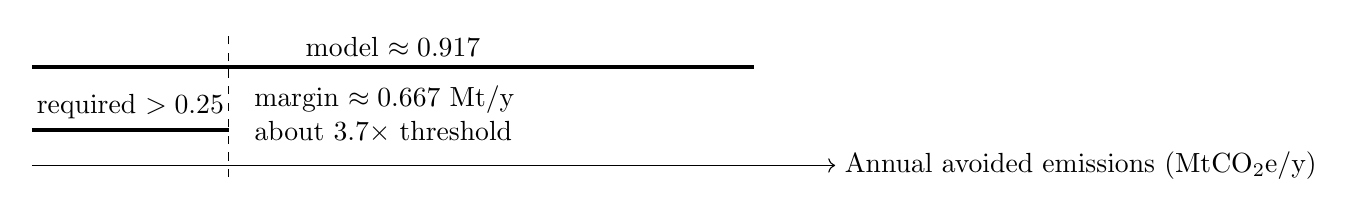
\begin{tikzpicture}[x=1cm,y=1cm]
\draw[->] (0,0)--(10.2,0) node[right]{Annual avoided emissions (MtCO$_2$e/y)};
\draw[very thick] (0,0.45)--(2.5,0.45) node[midway,above]{required $>0.25$};
\draw[very thick] (0,1.25)--(9.17,1.25) node[midway,above]{model $\approx0.917$};
\draw[dashed] (2.5,-0.15)--(2.5,1.65);
\node[align=left,anchor=west] at (2.7,0.65) {margin $\approx0.667$ Mt/y\\about 3.7$\times$ threshold};
\end{tikzpicture}
\caption{CN4252 annual-abatement test using the independently verified final lifecycle result. The model result is a conditional screening result, not measured project performance.}
\label{fig:abatement-threshold}
\end{figure}


\subsection{Economic robustness}
Abatement cost asks how much additional annual cost is associated with each tonne of lifecycle emissions avoided. Its definition is given by Eq.~\ref{eq:abatement-cost-definition}, and the full numerical substitution is Eq.~\ref{eq:abatement-cost-final}.
The controlling case gives no monetary credit to uncertain project electricity output but still charges the full selected reactor source-product economic burden. Its approximately S\$3.725/tCO$_2$e result is about S\$96.3/t below the S\$100/t ceiling. Thus the numerical cost pass does not depend on electricity revenue.

\begin{figure}[htbp]\centering
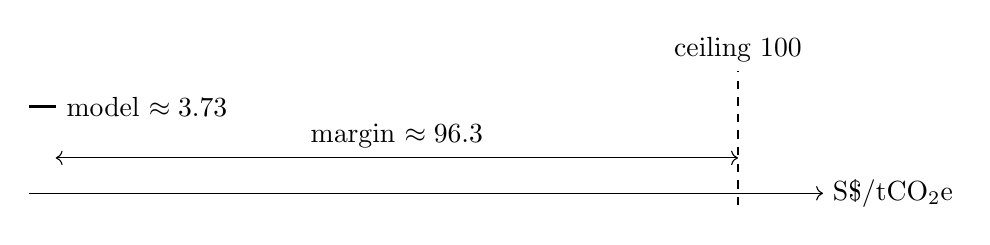
\begin{tikzpicture}[x=0.09cm,y=1cm]
\draw[->] (0,0)--(112,0) node[right]{S\$/tCO$_2$e};
\draw[very thick] (0,1.1)--(3.725,1.1) node[right]{model $\approx3.73$};
\draw[dashed] (100,-0.15)--(100,1.55) node[above]{ceiling 100};
\draw[<->] (3.725,0.45)--(100,0.45) node[midway,above]{margin $\approx96.3$};
\end{tikzpicture}
\caption{CN4252 abatement-cost test for the controlling zero-electricity-revenue case.}
\label{fig:cost-threshold}
\end{figure}


\subsection{Conditional model pass}
The final configuration satisfies both numerical assignment thresholds under the declared source/design-study and lifecycle assumptions. It remains a \textbf{CONDITIONAL MODEL RESULT}, not evidence of an existing Singapore commercial project.


\section{Deployment constraints and decision-gated implementation}\label{sec:deployment}

A promising equation is not a construction permit. Deployment is a sequence of tests in which a failure can force a smaller design, another site or cancellation. The roadmap below is a dependency chain, not a prediction of when Singapore will deploy nuclear power.

The preferred mature numerical case is not a deployment claim. Implementation follows the E7 falsification pathway:
\begin{enumerate}
\item Current research and evidence-gap closure.
\item Component and nuclear/process-interface qualification.
\item First-of-a-kind (FOAK) process-heat demonstration.
\item Two-train 353.6 MWth process-heat demonstration.
\item Replication and early-commercial (BOAK) cost validation.
\item Mature 10-OAK economic decision gate.
\item Singapore site, licensing and contract closure.
\item Construction and commissioning.
\item Commercial operation and measured verification.
\end{enumerate}
This sequence is a logical set of evidence gates, not a calendar schedule; failure at a gate requires redesign, relocation, delay or termination as appropriate.

\subsection{Binding implementation gates}
Before a real Singapore project can proceed, the following must close:
\begin{itemize}
\item \textbf{national/regulatory readiness:} an applicable power-reactor policy, competent regulator, licensing/legal framework, safeguards/security, waste/spent-fuel, EPR, liability and workforce arrangements;
\item \textbf{technology qualification:} 600 MWth coupled transients, high-temperature IHX/secondary-He/reformer qualification, tritium, controls/isolation, materials and inspection;
\item \textbf{two-train proof:} physical delivery of 353.6 MWth within the source process-heat branch, including one- and two-train trips, turndown, restart, CCS interaction and H$_2$ quality;
\item \textbf{integrated safety:} PRA, mechanistic source term, IHX leak/rupture, tritium, chemical HAZOP/QRA, propagation/common cause, UHS/SBO, dispersion/dose, EPR/EPZ and security;
\item \textbf{site/Jurong:} parcel, geotechnical/coastal/external hazards, QRA/PRA-derived separation, protected area, emergency access, cooling and environmental baseline;
\item \textbf{infrastructure/market:} credible H$_2$ offtake for approximately 195,892 t/y, firm 68 MMSCFD NG supply, water/cooling, and contracted permanent storage for at least approximately 1.085 MtCO$_2$/y;
\item \textbf{economic maturation:} observed replication cost, construction, operations and maintenance (O\&M), and integrated availability must support a recalculated cost below S\$100/tCO$_2$e, including known site, licensing, security and CCS costs;
\item \textbf{commercial/FID:} full project CAPEX/TCI, financing/IDC, insurance/liability, decommissioning/waste, EPC/owner costs and binding contracts.
\end{itemize}

Jurong failure does not automatically falsify the technology: another Singapore context may be evaluated. Conversely, if no Singapore context can satisfy siting, safety, security and emergency requirements, Singapore deployment is stopped.

\subsection{STOP/REDESIGN logic}
The project does not advance automatically. It is redesigned, relocated, reduced in scale, delayed or stopped if high-temperature coupling cannot be qualified; the two-train dynamics fail; integrated availability invalidates the model; observed mature economics remain at or above S\$100/tCO$_2$e; nuclear/chemical separation is infeasible; source-term/dose or external hazards are incompatible with a site; no credible UHS exists; H$_2$ offtake or the CCS chain cannot be contracted; or the future Singapore regulator rejects the design/site.

Only measured commissioning and commercial operation can convert the projected BOAK/10-OAK performance into demonstrated performance.

\section{Limitations}
The final process balance is anchored to INL Aspen studies rather than a project-owned detailed equipment simulation. The repository independently reconstructs annualisation, lifecycle extensions, helium-flow screening, deployment economics and CN4252 classification, but it does not reproduce INL's proprietary Aspen stream files. Reactor/IHX integration is screening-level: the 176.8 MWth final duty exceeds the 170 MWth reference GTHTR300C IHX, so the doubled-IHX cost sensitivity is used conservatively without claiming a completed exchanger design.

Upstream-gas, nuclear-lifecycle and CCS-transport factors are screening proxies rather than Singapore-specific measured inventories. Historical-cost escalation uses transparent broad deflators rather than nuclear-specific construction indices. Electricity value and T\&S remain scenarios, not guaranteed Singapore contracts. The mature GTHTR300C cost basis is a design-study estimate rather than an observed commercial plant cost. Nuclear licensing, siting, high-temperature process qualification and cross-border CCS remain future deployment conditions.

Accordingly, any CN4252 pass is a conditional model result under the declared literature/design-study assumptions. It does not establish bankable project feasibility or a technology preference over alternatives whose Singapore economics are not matched in this study.

\section{Nuclear engineering feasibility and safety}
\label{sec:nuclear-safety}

\subsection{Evidence maturity}
JAEA's 30 MWth HTTR is a constructed helium-cooled, graphite-moderated test reactor that achieved a 950$^\circ$C outlet temperature at full power~\cite{jaeahttr2026ops}. The selected 600 MWth GTHTR300C-class configuration is instead a design/economic architecture~\cite{nishihara2007potential}, while INL TEV-961 is a process model showing that 925$^\circ$C reactor outlet and 900$^\circ$C delivered heat can supply the 176.8 MWth reforming duty~\cite{inltev961}. The project therefore combines demonstrated temperature precedent, designed reactor architecture and modelled process integration; it does not claim a demonstrated 600 MWth nuclear-SMR plant.

\subsection{TRISO and passive/inherent characteristics}
\textbf{Plain-language takeaway:} each TRISO particle is a tiny fuel kernel wrapped in several engineered barrier layers; those layers strongly retain fission products, but they are not indestructible. TRISO fuel is a layered pressure vessel at particle scale. Around the fuel kernel, a porous carbon buffer accommodates fission gas and kernel swelling; the inner pyrolytic-carbon (IPyC, a dense carbon coating) layer provides structural support and protects the silicon-carbide deposition interface; dense silicon carbide (SiC, a ceramic barrier) is the principal pressure-bearing and metallic-fission-product barrier; and the outer pyrolytic-carbon (OPyC) layer provides additional mechanical/environmental protection~\cite{sawa2001httrfuel,sawaueta2004}. INL's AGR qualification programme adds modern UCO irradiation and post-irradiation safety evidence: 1600--1800$^\circ$C tests measured fission-product release and identified the consequences of SiC/coating failures~\cite{demkowicz2015facs,morris2016agr1,inlagrrelease}. Intact SiC showed excellent cesium retention in these tests, but measurable failure/release mechanisms remain; TRISO therefore reduces source-term potential (the amount of radioactive material available for release) rather than making radionuclide release impossible.

HTGR safety also uses reactor-scale physics. JAEA reports HTTR average power density of 2.5 MW/m$^3$ and a large graphite inventory~\cite{jaeahttr2026ops}. In the 9 MW HTTR loss-of-forced-cooling test, primary circulators were stopped without control-rod insertion; test/analysis evidence shows power falling rapidly toward decay heat through negative temperature-reactivity feedback while temperatures changed slowly because of graphite thermal inertia~\cite{takamatsu2011lofc}. These features reduce transient severity but do not remove the need for shutdown systems, decay-heat analysis, confinement, emergency planning or accident assessment.

\subsection{Accident mechanisms retained}
\textbf{Plain-language takeaway:} favourable HTGR physics does not remove accident analysis; loss of helium pressure, unwanted air or steam entry, loss of heat removal and radioactive-material transport still have to be evaluated. NRC HTGR/TRISO PIRTs explicitly retain depressurisation accidents with air ingress and water ingress, while the NGNP process-heat PIRT identifies intermediate-loop blowdown/loss of heat sink, leakage into the primary system and reactive-gas ingress as coupled-system safety phenomena~\cite{nrctriso6844,nrcngnppirt2010}. Depressurisation and subsequent air ingress can expose hot graphite to oxygen, so graphite oxidation and its effects on structural integrity remain accident mechanisms; fission-product transport during normal and accident conditions is itself a dedicated NRC PIRT topic~\cite{nrcngnpfpt2008}. Water/steam ingress, loss of heat sink and primary leakage likewise require design-specific analysis. The project therefore does not describe HTGRs as risk free or claim that severe fuel damage is impossible under every condition.

\subsection{IHX: heat-transfer equipment and safety boundary}
\textbf{Plain-language takeaway:} the IHX is both a heater and a physical separator; its metal boundary must survive high temperature for long periods without allowing the reactor and chemical loops to mix. JAEA's constructed HTTR IHX is a 10 MW helium--helium exchanger whose Hastelloy XR tubes form the pressure boundary between primary and secondary helium. Development work addressed creep collapse and creep-fatigue (slow high-temperature deformation combined with repeated thermal/mechanical cycling), seismic behaviour, bundle thermal hydraulics and in-service inspection~\cite{hamamoto2006ihx}. Structural analysis reports primary helium near 950$^\circ$C and secondary helium up to about 905$^\circ$C, with high-temperature creep explicitly governing design~\cite{httrihx1995}.

IAEA coupling guidance identifies the intermediate circuit as a means to separate the nuclear island from the chemical plant, limit radioactive contamination and reduce propagation of chemical disturbances into the reactor~\cite{iaeanuclearhydrogen2013}. This supports the project's primary-helium $\rightarrow$ IHX $\rightarrow$ secondary-helium $\rightarrow$ reformer architecture. It does not remove scale-up work: a constructed 10 MW IHX and a designed 370 MWth source heat branch are not a completed 176.8 MWth project exchanger.

\subsection{Coupled nuclear--chemical transients}
\textbf{Plain-language takeaway:} if one plant suddenly changes state, the other must not be driven into an unsafe condition; ``propagation'' here means one plant's disturbance causing a consequential event in the other. A chemical-plant trip or rapid heat-demand change alters secondary-helium return conditions. IAEA/JAEA work identifies return-helium control and prevention of reactor trips as explicit integration-development needs~\cite{iaeacoupling2009}. Conversely, reactor trip or loss of nuclear heat requires the chemical plant to reach a safe state with hot, pressurised methane/steam/hydrogen inventories. Independent trips, isolation, secondary-loop thermal management and process depressurisation therefore require future transient design; this screening study does not size those systems.

\subsection{Chemical/process hazards and co-location}
The hydrogen plant introduces combustible hydrogen and methane, toxic carbon monoxide, hot high-pressure syngas/steam, reformer fire/explosion hazards, solvent/capture equipment and compressed CO$_2$. A future process hazard analysis must evaluate leakage, ignition, explosion overpressure, toxic/asphyxiant releases, escalation and loss of utilities. The NRC NGNP process-heat/hydrogen PIRT emphasises chemical inventories, layout and separation distance as major controls against propagation to the nuclear plant~\cite{nrcngnppirt2010}; IAEA work likewise identifies combustible leakage/explosion as an HTGR-hydrogen integration issue~\cite{iaeacoupling2009}.

\subsection{Safety-feasibility conclusion}
At screening level the design has a credible physical safety architecture: TRISO fuel, graphite/helium HTGR characteristics, an intermediate helium boundary and demonstrated high-temperature IHX precedent. \textbf{Safety feasibility remains conditional}: site-specific accident consequences, chemical-to-nuclear propagation limits, separation distances, detailed IHX integrity, emergency planning and regulatory acceptance are not demonstrated here.
\section{Singapore implementation implications}
The corrected model translates the candidate into annual H2, fresh-NG energy, captured/residual CO2, cross-border storage throughput, nuclear process heat and helium-loop scale. Required thermal service is expressed against the source-backed 170 MW JAEA IHX benchmark rather than converted into a fabricated commercial reactor-module count.

Singapore deployment remains conditional~\cite{singaporenuclear,singaporeccs}. Nuclear power has not been assumed to be deployed, and cross-border CO2 transport/storage is treated as infrastructure under development rather than an existing domestic storage service. An implementation roadmap would therefore require, at minimum, nuclear regulatory/readiness development, site and safety assessment, a demonstrated process-heat coupling architecture, and contracted cross-border CO2 transport/storage.


\section{Conclusions}
The final chemical-process basis remains the INL/NGNP high-temperature nuclear-assisted SMR+CCS case: 130 MMSCFD H$_2$, 871$^\circ$C reforming, 176.8 MWth nuclear process heat and 17.3 MWe process demand~\cite{inltev953,inltev961}. At 85\% availability the declared lifecycle boundary gives approximately 0.917 MtCO$_2$e/y avoided, well above the CN4252 annual threshold.

The corrected hardware/economic calculation uses one coherent Nishihara GTHTR300C source architecture rather than mixing JAEA variants. The source split is 370 MWth hydrogen heat plus a 230 MWth power branch producing 88 MWe; the project's 176.8 MWth process draw is mapped explicitly to the residual reactor branch. Under that screening mapping, the zero-electricity-value case remains below S\$100/tCO$_2$e, while electricity-value cases provide additional sensitivities.

The resulting joint pass is a \textbf{conditional model result pending independent reviewer re-verification}. It is not a claim of demonstrated Singapore commercial feasibility or a guaranteed electricity offtake. The INL process design, JAEA hardware/economic source case and project-derived integration quantities are kept explicitly distinct.

\appendix
\section{Reproducibility}
From a fresh repository checkout, the canonical end-to-end reproduction command is:
\begin{verbatim}
sh paper/build.sh
\end{verbatim}
The build script runs the complete Rust test suite, regenerates the canonical Gate-5/Gate-6 manuscript datasets, invokes \texttt{latexmk}, and fails if unresolved LaTeX citations or references remain. For explicit verification, the equivalent sequence is:
\begin{verbatim}
cd model
cargo test --all-targets
sh scripts/generate_gate5_results.sh
cd ../paper
latexmk -pdf -interaction=nonstopmode -halt-on-error main.tex
\end{verbatim}

The Rust implementation in \texttt{model/src/lib.rs} is the canonical computational source. Generated CSV/Markdown files under \texttt{results/generated/} are derivative artifacts and are recreated during the paper build. The quantitative manuscript chain is therefore:
\[
\text{source/assumption}
\rightarrow \text{Rust model}
\rightarrow \text{generated CSV}
\rightarrow \text{LaTeX table/figure}
\rightarrow \text{PDF}.
\]
The PDF is generated from \texttt{paper/main.tex} and is never maintained independently.

The GitHub Actions paper workflow invokes this same canonical build script on a fresh runner, avoiding a separate CI-only reproduction path. A successful current workflow run, rather than the existence of a locally generated PDF alone, is the Gate-6 reproducibility acceptance evidence.

\section{CN4252 requirement traceability}
\begin{center}
\begin{tabular}{p{0.31\linewidth}p{0.55\linewidth}}
\toprule
Requirement & Manuscript evidence \\
\midrule
$>0.25$ MtCO2e/y & Sections 7--9: 64-case threshold experiment, Eq.~\eqref{eq:joint-pass}, and Case-1A common-scale comparator. \\
$<$S\$100/tCO2e & Sections 4, 7--9: Eqs.~\eqref{eq:annual-avoided}--\eqref{eq:abatement-cost}, threshold map and falsification results. \\
Show how emissions are abated & Sections 3, 4 and 6: reforming/CCS/recycle/heat/lifecycle boundary. \\
Implementation roadmap & Section 10: conditional nuclear readiness and cross-border CCS requirements. \\
Feasibility, effectiveness and accuracy & Sections 5, 7--13: verification, uncertainty, comparator evidence and limitations. \\
\bottomrule
\end{tabular}
\end{center}

\bibliographystyle{unsrtnat}
\bibliography{references}
\end{document}
